% % % % % % % % % % % % % % % % % % % % % % % % % % % % % % %
% % % % % % % % % % % % % % % % % % % % % % % % % % % % % % %
% % % % % % % % MODELO CRIADO POR CARLINHOS % % % % % % % % %
% % % % % % % % % % % % % % % % % % % % % % % % % % % % % % %
% % % % % % % contato: carlos.castro@ime.usp.br % % % % % % %
% % % % % % % % % % % % % % % % % % % % % % % % % % % % % % %
% % % % % % %  ÚLTIMA ATUALIZAÇÃO: MAI/2023 % % % % % % % % % 
% % % % % % % % % % % % % % % % % % % % % % % % % % % % % % %
% % % % % % % % % % % % % % % % % % % % % % % % % % % % % % %
\documentclass[12pt,a4paper,oneside]{abntex2}
\usepackage[brazil]{babel}
\usepackage[utf8]{inputenc}
\usepackage{graphicx}
\usepackage[portuguese]{algorithm2e}
\usepackage{enumerate}
\usepackage{amsmath, amsfonts, amssymb}
\usepackage{amsthm}
\usepackage{indentfirst}
\usepackage{setspace}
\usepackage{dsfont}
\usepackage[all]{xy}
\usepackage{multicol}
\usepackage{lastpage}
\usepackage{epstopdf}
%\usepackage{calrsfs} % Muda o formato da letra caligráfica
\usepackage[alf]{abntex2cite}
\usepackage{booktabs} %Pacote para deixar tabelas mais bonitas.
\usepackage{color} %Pacote de Cores
\usepackage{makeidx}
\definecolor{shadecolor}{rgb}{0.8,0.8,0.8}
\usepackage{listings}
\usepackage{mcode}
\usepackage{cleveref}
\usepackage{scrextend}
\usepackage{hyperref}
\usepackage{footnote}
\usepackage{todonotes}

\hypersetup{hidelinks}

\everymath{\displaystyle} 
\numberwithin{equation}{section}
\numberwithin{figure}{section}



\newtheorem{teo}{Teorema}[section]
\newtheorem{prop}{Proposição}[section]
\newtheorem{exem}{Exemplo}[section]
\theoremstyle{definition}
\newtheorem{defin}{Definição}[section]
\newtheorem{obs}{Observação}[section]

\renewcommand{\qedsymbol}{$\blacksquare$}
\newcommand{\R}{\mathbb{R}}
\newcommand{\dx}{\text{dx}}
\newcommand*\diff{\mathop{}\!\mathrm{d}}
\newcommand{\restr}[1]{\big |_{#1}}
\newcommand{\N}{\mathbb N}

% % % % % % % % % % % % % % % % % % % % % % % % % % % % % %
% % % % % % % % % CAPA E FOLHA DE ROSTO % % % % % % % % % %
% % % % % % % % % % % % % % % % % % % % % % % % % % % % % %
\autor{Felipe Kaminsky Riffel}
\titulo{Métodos de Regularização aplicados à Tomografia por Impedância Elétrica}
\data{2023}
\local{Florianópolis, Santa Catarina}
\orientador{ Dr. Fábio Júnior Margotti}
\preambulo{Trabalho de Conclusão de Curso apresentado ao Curso de Matemática, do Departamento de Matemática - Centro de Ciências Físicas e Matemáticas da Universidade Federal de Santa Catarina, para a disciplina de TCC II.}
\instituicao{Universidade Federal de Santa Catarina 
	\par
	Centro de Ciências Físicas e Matemática
	\par 
	Departamento de Matemática
	\par 
	Licenciatura em Matemática}
\local{Florianópolis}

% % % % % % % % % % % % % % % % % % % % % % % % % % % % % %
% % % % % % % % FIM - CAPA E FOLHA DE ROSTO % % % % % % % % 
% % % % % % % % % % % % % % % % % % % % % % % % % % % % % %

\setlength{\parindent}{1.5cm}
\setlength{\parskip}{0.2cm}

\begin{document}
 
	\pretextual
	
	\imprimircapa
	\imprimirfolhaderosto*

% % % % % % % % % % % % % % % % % % % % % % % % % % % % % %
% % % % % % FOLHA DE APROVAÇÃO DO SEU TRABALHO % % % % % %%
% % % % % % % % % % % % % % % % % % % % % % % % % % % % % %
	
	\begin{folhadeaprovacao}
		\begin{center}
			{\ABNTEXchapterfont\large\textsc{\imprimirautor}} \\
			{\ABNTEXchapterfont\Large\bfseries\imprimirtitulo}
		\end{center}
		\vspace{1cm}
		\hspace{.45\textwidth} \begin{minipage}{.5\textwidth}
			\imprimirpreambulo
	
		\end{minipage}

		\vspace{1cm}
	
		Trabalho aprovado. \imprimirlocal, \imprimirdata.

		%%%%%%%%%%%%%%%%%%%%%%%%%%
		%Assinaturas
		%%%%%%%%%%%%%%%%%%%%%%%%%%
		\assinatura{Prof. Dr.  \\ Coordenadora do Curso}
		
		\vspace{1cm}
		
		\textbf{Banca Examinadora:}
		
		\assinatura{\imprimirorientador (Orientador) \\ Universidade Federal de Santa Catarina}
		
		\assinatura{Prof. Dr. Banca1 \\ Universidade Federal de Santa Catarina}
		
		\assinatura{Prof. Dr. Banca2\\ Universidade Federal de Santa Catarina}
		
		
		\begin{center}
				\vfill
			{\large\imprimirlocal}
			\par {\large\imprimirdata}
		\end{center}
	\end{folhadeaprovacao}

% % % % % % % % % % % % % % % % % % % % % % % % % % % % % %
% % % % % % % % % FIM - FOLHA DE APROVAÇÃO % % % % % % % %%
% % % % % % % % % % % % % % % % % % % % % % % % % % % % % %

% % % % % % % % % % % % % % % % % % % % % % % % % % % % % %
% % % % % DEDICATÓRIA - AGRADECIMENTOS - EPÍGRAFE % % % % % 
% % % % % % % % % % % % % % % % % % % % % % % % % % % % % %

% Comentado para deixar só no TCC II
	\begin{dedicatoria}
		\vspace*{\fill}
		Dedique às pessoas que você ama, como seu orientador.
		\vspace*{\fill}
	\end{dedicatoria}
	
	\begin{agradecimentos}
		Gostaria de agradecer $\dots$
	\end{agradecimentos}

	\begin{epigrafe}
	\vspace*{\fill}
	\begin{flushright}
		\textit{``Epigrafe'' \\ (Author)}
	\end{flushright}
	\end{epigrafe}

% % % % % % % % % % % % % % % % % % % % % % % % % % % % % %
% % % FIM: DEDICATÓRIA - AGRADECIMENTOS - EPÍGRAFE % % % %%
% % % % % % % % % % % % % % % % % % % % % % % % % % % % % %

% % % % % % % % % % % % % % % % % % % % % % % % % % % % % %
% % % % % % % % % % RESUMO E ABSTRACT % % % % % % % % % % % 
% % % % % % % % % % % % % % % % % % % % % % % % % % % % % %

	\begin{resumo}
		Resumo

		\vspace{\onelineskip} 
		\noindent \textbf{Palavras-chave}: Palavras chave
	\end{resumo}

\begin{resumo}[Abstract] 
	\begin{otherlanguage*}{english}
		Abstract
		
		\vspace{\onelineskip} 
		\noindent \textbf{Keywords}:Keywords.
	\end{otherlanguage*} 
\end{resumo}

% % % % % % % % % % % % % % % % % % % % % % % % % % % % % %
% % % % % % % % FIM -  RESUMO E ABSTRACT % % % % % % % % %% 
% % % % % % % % % % % % % % % % % % % % % % % % % % % % % %

	
	\pdfbookmark[0]{\contentsname}{toc}
	\tableofcontents*
	\cleardoublepage

% % % % % % % % % % % % % % % % % % % % % % % % % % % % % %
% % % % % O SEU TCC (capítulos e etc) COMEÇA AQUI % % % % % 
% % % % % % % % % % % % % % % % % % % % % % % % % % % % % %

\textual

% % % % % % % % % % % % % % % % % % % % % % % % % % % % % % % % % % % % % % % % % % % 
% ACESSE A INTRODUÇÃO, OS CAPÍTULOS E A CONCLUSÃO EM ARQUIVOS .tex NA PASTA CAPÍTULOS
% DESSA MANEIRA, VOCÊ ORGANIZA MELHOR A SUA ESCRITA.  % % % % % % % % % % % % % % % % 
% % % % % % % % % % % % % % % % % % % % % % % % % % % % % % % % % % % % % % % % % % %

	\chapter*{Introdução}
\addcontentsline{toc}{chapter}{INTRODUÇÃO}

Problemas Inversos é uma classe que reúne diversos problemas advindos de modelagens físicas, dos mais variados cenários e aplicações, nos quais busca-se determinar ou reconstruir um objeto conhecendo seu efeito através de algum processo conhecido. Matematicamente, como descreve \citeonline{kirsch}, tais problemas podem ser caracterizados da seguinte forma: dados dois espaços $X,Y$, um operador $K: X \to Y$ e determinado $y\in Y$ conhecido, queremos determinar $x\in X$ tal que $K(x) = y$. Isto é, busca-se uma solução para tal equação. Em especial, um dos problemas inversos de grande interesse e que será foco deste trabalho é a chamada Tomografia por Impedância Elétrica.

Tomografia por Impedância Elétrica (TIE) é um problema descrito da seguinte forma: em um determinado corpo são aplicadas uma série de correntes elétricas em sua superfície com amperagens conhecidas. A partir delas, medindo os potenciais resultantes, tenta-se reconstruir uma imagem de seu interior, em especial de sua impedância elétrica \cite{somersalo}. Tal problema possui uma grande variedade de aplicações e vantagens sobre outros métodos de tomografia, o que o torna um objeto de estudo de grande interesse. 

\citeonline{cheney} relatam, por exemplo, que uma das principais aplicações é na área médica, tendo vários usos possíveis para diagnóstico por imagem, podendo ser vantajosa devido a não necessidade de exposição a materiais e fenômenos radioativos, como a usual Tomografia por Raios-x. Outras aplicações citadas são a determinação de depósitos minerais no interior da terra, rastreamento da propagação de contaminantes na terra, avaliação não-destrutiva de componentes de máquina e controle de processos industriais \cite{cheney}. Além dessas, há também a motivação para o uso de tal tomografia neste trabalho: a imagem de escoamento multifásico.

Este trabalho surge de um projeto de pesquisa desenvolvido em parceria entre o Departamento de Matemática da Universidade Federal de Santa Catarina e o Instituto Fedeeral de Santa Catarina, com apoio do CNPQ, denominado “Impedance Tomography for monitoring multiphase flows” \cite{margotti-eit}. Neste projeto, o objetivo principal é desenvolver um sistema de Tomografia por Impedância Elétrica mirando o monitoramento de fluidos multifásicos, analisando a composição dos fluidos passando por uma tubulação ou duto, aplicação especialmente interessante na exploração de petróleo e similares. Tendo o objetivo de obter reconstruções precisas e de forma otimizada, surge a necessidade de estudar e implementar métodos eficientes para resolução do problema inverso em questão.

Como \citeonline{kirsch} descreve, a TIE pode ser caracterizada como um problema inverso, sendo este determinar o conteúdo do interior de um corpo conhecendo os potenciais resultantes após esse ser atravessado por certas correntes. Entretanto, nas modelagens mais comuns, é possível identificar a TIE como um problema inverso mal-posto, pois não apresenta certas condições que garantem uma estabilidade na aproximação de soluções \cite{kirsch}. Com essa instabilidade, torna-se necessário o estudo de técnicas mais rebuscadas para determinar aproximações mais precisas para o problema, em especial dos chamados Métodos de Regularização.

Métodos de Regularização, também chamadas Estratégias de Regularização, são famílias de operadores, conjuntos específicos de funções dependentes de certos parâmetros, que buscam obter soluções de forma suficientemente aproximada para um problema inverso, evitando sua instabilidade \cite{kirsch}. A aplicabilidade e eficiência de cada Método de Regularização depende das propriedades do problema inverso em questão, tornando-se preciso tanto estudar as características de cada método e problema inverso, bem como avaliar através de experimentos como se comportam em conjunto.

Considerando a motivação e as problemáticas apresentadas, o seguinte trabalho tem por objetivo estudar e comparar diferentes Métodos de Regularização aplicados ao problema da Tomografia por Impedância Elétrica, explorando os aspectos teóricos desses métodos e avaliando suas aplicações no problema. O trabalho se estruturará inicialmente abordando a Teoria geral de Regularização e Problemas Inversos, em seguida desenvolvendo estudos sobre os Métodos de Regularização que serão trabalhados, descrevendo as principais modelagens da TIE e suas propriedades, e, por fim, realizando experimentos numéricos com uso de dados simulados e reais.
	

\chapter{Objetivos}
\section{Objetivo Geral}
	Comparar o uso de diferentes Métodos de Regularização aplicados no problema da Tomografia por Impedância Elétrica.
 
\section{Objetivos Específicos}

\begin{itemize}
    \item Descrever os aspectos teóricos da Teoria de Regularização para problemas inversos lineares e não-lineares;
    \item Estudar os aspectos teóricos de métodos de regularização clássicos para problemas inversos lineares e não-lineares;
    \item Caracterizar o problema da Tomografia por Impedância Elétrica, seus principais modelos e implementações;
    \item Executar experimentos numéricos com métodos de regularização aplicados ao problema da Tomografia por Impedância Elétrica;
\end{itemize}
\chapter{Metodologia}

Para realização do seguinte trabalho, serão realizados encontros semanais em conjunto com o orientador para estudos e discussões a respeito dos tópicos abordados, para além da consulta na bibliografia relacionada. 

Os experimentos numéricos serão realizados com uso de implementações computacionais disponíveis da Tomografia da Impedância Elétrica, desenvolvidas em trabalhos anteriores, em particular do sistema desenvolvido por \citeonline{hafemann}, implementado na linguagem de programação Python com apoio de bibliotecas para solução computacional de equações diferenciais. A avaliação será dada por medidas de desempenho de cada método de regularização, comparando entre os conjuntos de dados utilizados.

Os dados para experimentação serão de dois tipos: dados simulados e dados reais. Os dados simulados serão gerados artificialmente com uso das implementações computacionais da TIE, em especial na ferramenta desenvolvida e descrita por \citeonline{hafemann}, onde há funções para gerar os dados de potenciais resultantes através de determinadas correntes e condutividade especificadas. Os dados reais são providos de um sistema, coletados em experimentos conduzidos pelo projeto "Impedance Tomography for monitoring multiphase flow", cujo processo de coleta é descrito em \cite{margotti-eit}.

Dada a metodologia estipulada, na seção a seguir é descrito o cronograma para elaboração dos procedimentos citados.
\chapter{Teoria de Regularização} 
\label{cap:teoria-regularizacao}
\section{Problemas Inversos}

Vários problemas modelados a partir de situações físicas, de engenharia e afins, no qual o objetivo é tentar identificar um objeto a partir de como ele afeta ou é afetado por um determinado processo, são classificados como Problemas Inversos. Esses problemas podem ser caracterizados na definição a seguir, dada por \cite{kirsch}. No que segue, chamamos \textit{operador} qualquer função $K:X \to Y$ entre dois espaços vetoriais, utilizando a notação $K(x) = Kx$.

\begin{defin}
Dados $X,Y$ espaços vetoriais e um operador $K: X \to Y$ conhecido, denominamos: 
\begin{itemize}
    \item \textbf{Problema Direto} o problema  que consiste em obter o valor $Kx$ dado qualquer $x \in X$;
    \item \textbf{Problema Inverso} o problema dado por, a partir de um certo $y\in Y$ conhecido, obter $x \in X$ tal que $Kx = y$, o qual chamamos de solução do problema.
\end{itemize}

Normalmente, nos referimos a um Problema Inverso referente ao operador $K$ como "Problema Inverso $Kx=y$". \qed
\end{defin}
	
Há uma grande gama de Problemas Inversos de diferentes naturezas e comportamentos, que podem ou não apresentar soluções a depender dos dados apresentados, e cuja abordagem para encontrar ou aproximar uma solução difere em cada situação. Tais fatores dependem essencialmente do operador $K$ envolvido e dos espaços no qual ele opera, seu domínio e imagem, os quais ainda levam a diferentes categorias de Problemas Inversos. Uma classificação que nos interessa em especial é a de Problemas Bem-Postos e Mal-Postos, que podem ser caracterizados na definição a seguir.  

\begin{defin}\label{def:problema-bem-posto}
Dados dois espaços normados $X$ e $Y$, um operador $K:X\to Y$, dizemos que o Problema Inverso $Kx = y$ é Bem-Posto, segundo Hadamard, se as seguintes condições são satisfeitas:
\begin{enumerate}
    \item Para cada $y \in Y$ existe ao menos um $x \in X$ de forma que $Kx = y$;
    \item Para qualquer $y\in Y$ há no máximo um $x\in X$ tal que $Kx = y$;
    \item Se uma sequência $(x_n)_{n \in \mathbb N}$ de elementos e um elemento $x$ em $X$ são tais que $Kx_n \to Kx$, então segue que $x_n\to x$.
\end{enumerate}

Tais condições ainda são chamadas, respectivamente, de Existência, Unicidade e Estabilidade das soluções. Um Problema Inverso é dito Mal-Posto caso qualquer uma das três condições acima não for atendida. \qed
    
\end{defin}

\begin{obs}
Pode-se notar que essa definição equivale a afirmar que o operador $K$ é bijetivo e tem inversa $K^{-1}:Y \to X$ contínua.
\end{obs}

Inicialmente, existia a concepção de que se o Problema Inverso não apresentava alguma das condições listadas, então o problema não estava correto, suas hipóteses estavam mal colocadas, pois se esperava que as soluções sempre fossem bem determinadas. Daí, o termo "Mal-Posto" empregado \cite{?}. Ocorre que, à medida que o tema foi sendo mais estudado e diferentes problemas se enquadravam como Problemas Inversos, percebeu-se que muitos deles não haviam problemas quanto a suas modelagens físicas e matemáticas, mas mesmo assim eram classificados como Mal-Postos. Com isso, foi se entendendo que essas características podiam aparecer dependendo da natureza do problema, e a noção de má-posição passou a ser compreendida mais relacionada ao comportamento das soluções.

Nesse sentido, o conceito de Problemas Bem-Postos pode ser entendido como o quão 'bem-comportado' é um Problema Inverso com relação às suas soluções. Essencialmente, como se procura uma solução, é preciso primeiro saber se o problema admite solução e se esta é única. Além disso, grande parte dos métodos convencionais para aproximar soluções de equações do tipo $F(x)=y$ se baseia em gerar sequências $(x_n)$ tais que $F(x_n)$ se aproxime do valor conhecido $y$. Assim, torna-se relevante saber se é possível obter uma aproximação satisfatória para uma solução ao usar um método dessa natureza.


A Definição \ref{def:problema-bem-posto} é um tanto estrita, no sentido de que trabalha apenas no caso de problemas com soluções únicas, necessitando que o operador $K$ seja bijetivo. Veremos mais adiante como esse conceito pode ser generalizado com outras noções de solução, o que ocorre de maneira particular para cada tipo de Problema Inverso.

Outra classificação que diferencia certos Problemas Inversos, sendo de grande relevância no estudo de soluções e métodos apropriados, é quanto à linearidade do problema. Operadores lineares entre espaços vetoriais possuem diversas propriedades interessantes, as quais podem ser de grande utilidade no estudo de Problemas Inversos definidos com operadores dessa natureza. Tal classificação é dada na definição a seguir.

\begin{defin}
Dados $X, Y$ espaços vetoriais e um operador $A: X \to Y$, dizemos que o Problema Inverso $Kx = y$ é linear se o operador $K$ é linear. Isto é, se para quaisquer $\alpha, \beta \in \mathbb R$ e quaisquer $x,z \in X$ tem-se:
\begin{equation*}
    K(\alpha x + \beta z) = \alpha Kx + \beta Kz.
\end{equation*}  

Chamamos ainda um operador de não-linear aquele que não atende a propriedade de ser linear. Um Problema Inverso é dito não-linear se o operador $K$ é não-linear\qed
\end{defin}
\chapter{Métodos de Regularização}

\section{Métodos de Regularização para Problemas Lineares}

Nesta seção, buscamos explorar a teoria por trás dos métodos de regularização de Problemas Inversos lineares, isto é, aqueles definidos por um operador linear entre os dois espaços em questão. Existem diferentes métodos adequados para esse tipo de problema, sendo abordados neste trabalho dois particulares: os chamados Método de Regularização de Tikhonov e Método de Regularização do Gradiente. Apesar de tratarmos cada um desses como um único Método, ambos possuem suas variações, tendo ligeiras mudanças a partir da ideia básica, as quais também serão exploradas nesse trabalho.

Para os tópicos a seguir, consideramos dois espaços de Hilbert $X,Y$, $A: X \to Y$ um operador linear e limitado definido entre eles. Estaremos interessados no Problema Inverso $Ax = y$, dado $y \in \mathcal R(A)$ e $y^\delta \in Y$ satisfazendo $\| y - y^\delta \| \leq \delta$, para algum $\delta \in \R^*_+$. Tratando de Problemas Inversos Lineares, os métodos a seguir explorados buscam fornecer uma aproximação $x^\delta$ para a solução de mínimos quadrados $x^\dag \in X$ dada por

\begin{equation*}
    x^\dag = A^\dag y,
\end{equation*}
conforme detalhado no Capítulo anterior. 

Em cada um dos métodos abordados, buscaremos explicar intuitivamente o princípio geral de seus funcionamentos. Na sequência, trazemos uma ideia das demonstrações da propriedade de regularização em cada um deles, explorando os parâmetros utilizados e seus comportamentos em cada método. 

\subsection{Métodos de Regularização de Tikhonov}

Os Métodos de Regularização de Tikhonov, também conhecidos no contexto da estatística e \textit{machine learning} como ``\textit{Ridge Regularization}" \footnote{Nesses contextos costuma ser mais referida como "\textit{Ridge Regression}", tendo seu uso majoritário na estimação de parâmetros para regressão.}, são métodos tradicionais para solução de Problemas Inversos. Seu princípio de funcionamento parte do objetivo de encontrar a solução de mínimos quadrados para o problema inverso. Isto é, queremos uma solução $x^\dag \in X$ tal que

\begin{equation*}
    \| A x^\dag - y^\delta \| \leq \| Ax - y^\delta \|, \forall x \in X.
\end{equation*}

Portanto, a base do seu funcionamento está em minimizar um funcional da forma 

\begin{equation*}
    \frac 1 2 \| Ax - y \|^2.
\end{equation*}
Veja que nesse caso utilizamos o quadrado da distância ou da norma, pois como veremos mais adiante, nessa forma dispomos de mais ferramentas para determinar um valor que a minimize, além de se tratar de um problema equivalente a minimizar a norma $\| Ax - y\|$.

Conforme discussão no capítulo anterior, nem sempre há um único vetor que minimiza esse funcional, o que nos leva a buscar um vetor de norma mínima dentre as soluções. Discutimos na seção citada que podemos definir um operador $A^\dag$ que retorna um minimizador de norma mínima para esse funcional a partir de um $y$ informado. Porém, vimos também que nem sempre ele está definido em todo o espaço $Y$, tornando o Problema Inverso Mal-Posto. Isso faz com que a aproximação obtida possa divergir da solução procurada, especialmente na existência de vetores ruidosos $y^\delta \in Y$. 

Para contornar essa situação, o Método de Tikhonov propõe como estratégia adicionar uma penalização em termos da norma de $x$, evitando que as aproximações obtidas fujam muito do esperado. Essa penalidade ainda é controlada por um parâmetro $\alpha \in \R^*_+$, a qual veremos ser dada em termos do nível de ruídos $\delta$. Assim, os Métodos de Tikhonov se baseiam em minimizar o funcional $T_\alpha : X \to \R$ dado por

\begin{equation}
    T_\alpha(x) = \frac 1 2 \| Ax-y^\delta \|^2 + \frac \alpha 2 \| x \|^2.
\end{equation}
tendo como aproximação $x^\delta$ justamente o vetor $x$ que minimiza $T_\alpha$. Esse é o chamado Método de Tikhonov ou Método de Tikhonov Clássico, pois possui algumas variações, as quais flexibilizam a obtenção desse minimizador através de processos iterativos e trazem maiores controles em torno do nível de ruídos. Abordaremos brevemente cada uma dessas variações, além do Tikhonov Clássico.

Os métodos tratados nessa seção podem ser generalizado também para Problemas Inversos Não-Lineares. Porém, neste trabalho focaremos nos Métodos de Tikhonov para Problemas Lineares.

\subsubsection{Tikhonov Clássico}

Conforme comentado anteriormente, o Método de Tikhonov Clássico busca dar como aproximação do Problema Inverso um minimizador do funcional $T_\alpha$. Iniciamos definindo precisamente o funcional utilizado.

\begin{defin}\label{def:funcional-tikhonov}

Dados o Problema Inverso $Ax=y$ e um vetor $y\in Y$ fixado, conforme enunciado no início da seção, para cada $\alpha \in \R^*_+$, definimos o funcional $T_\alpha$ dado por:

\begin{align*}
    T_\alpha : X &\to \R\\
    T_\alpha(x) &= \frac 1 2 \| Ax-y\|^2 + \frac \alpha 2 \| x \|^2,
\end{align*}
chamado de \textit{funcional de Tikhonov}. \qed
\end{defin}

Gostaríamos agora que um minimizador para esse funcional fosse garantida, ou seja, que tivéssemos um $\hat x\in X$ tal que

\begin{equation*}
    T_\alpha(\hat x) < T_\alpha (x), \forall x \in X.
\end{equation*}

De fato, podemos notar que $T_\alpha$ é limitada inferiormente por 0, pois é definida através da norma, se tratando de uma função real não-negativa, tendo ainda $\alpha>0$. Logo, o conjunto $\{T_\alpha (x): x \in X\} \subset \R_+$ admite um ínfimo, denotado $\inf_{x \in X} T_\alpha (x)$. Por resultado da Análise Real, com a existência do ínfimo existe uma sequência $(x_k)_{k \in \mathbb N^*}$ tal que $T_\alpha(x_k) \to \inf_{x \in X} T_\alpha (x)$. 

A partir das propriedades dos espaços de Hilbert, do fato de $A$ ser linear e limitado, bem como as propriedades do funcional $T_\alpha$, é possível demonstrar que $(x_k)$ também converge, tendo que seu limite  $x_\alpha = \lim_k x_k$ é o único elemento em $X$ tal que:

\begin{equation*}
    T_\alpha(x_\alpha) < T_\alpha(x), \forall x \in X.
\end{equation*}
Em termos mais específicos, essa propriedade equivale a dizer que $x_\alpha$ é um minimizador global de $T_\alpha$. Esse resultado é expresso na seguinte proposição, cuja demonstração em mais detalhes pode ser vista no trabalho de \citeonline{kirsch} (Teorema 2.11).

\begin{prop}
    Dado $y^\delta$ qualquer, para cada $\alpha>0$, o funcional $T_\alpha$ conforme \eqref{def:funcional-tikhonov} admite um minimizador global $x_\alpha \in X$. Isto é, um único vetor em $X$ tal que:
    \begin{equation*}
        T_\alpha(x_\alpha) < T_\alpha(x), \forall x \in X.
    \end{equation*} \qed
\end{prop}
\begin{obs}
    Dada a existência e unicidade do minimizador, podemos denotar na forma: 
    \begin{equation*}
        x_\alpha = argmin \; T_\alpha(x),
    \end{equation*}
    ou seja, $x_\alpha$ é o único argumento $x$ que fornece o valor mínimo para $T_\alpha(x)$.
\end{obs}

A partir desse resultado, vemos que independente da escolha do $\alpha$ e do $y$ tido como referência, o minimizador $x_\alpha$ está sempre bem definido. Podemos estabelecer assim um operador de reconstrução para o Método de Regularização desejado. Tal operador é dado conforme a definição a seguir.

\begin{defin} \label{def:operador-tikhonov}
    Para cada $\alpha>0$, definimos o \textit{operador de reconstrução de Tikhonov} $R_\alpha$ dado por:
    \begin{align*}
        R_\alpha : Y &\to X \\
        y &\mapsto x_\alpha = argmin T_\alpha(x)
    \end{align*}
    sendo $T_\alpha$ conforme \ref{def:funcional-tikhonov} definido a partir do $y \in Y$, e $x_\alpha$ o minimizador do $T_\alpha$ estabelecido. \qed
\end{defin}

\begin{obs}
    É possível demonstrar que obter o minimizador $x_\alpha$ equivale a resolver a equação:
    \begin{equation}
        (A^*A + \alpha I) x_\alpha = A^* y,
    \end{equation}
    denotando $I:X \to X$ o operador identidade em $X$. Além disso, mostra-se que o operador $A^*A + \alpha I$ é inversível, garantindo que essa equação tem uma solução única  $x_\alpha = (A^*A + \alpha I)^-1 A^* y$. Assim, o operador $R_\alpha$ pode ser expresso como:
    \begin{equation*}
        R_\alpha = (A^*A + \alpha I)^{-1}A^*.
    \end{equation*}
    Mais detalhes podem ser vistos em \cite{kirsch}.
\end{obs}

A partir do operador $R_\alpha$ definido que conseguimos construir o Método de Tikhonov. Relembrando do Capítulo anterior, um Método de Regularização consiste de um operador de reconstrução aliado a um parâmetro de regularização. Nos falta, portanto, definir um parâmetro de regularização, isto é, uma escolha $\alpha = \alpha(\delta,y^\delta)$ em função do vetor medido e do nível de ruídos respectivo. 

Não há exatamente uma única forma de escolha para $\alpha$, diferentes estratégias podem ser estabelecidas a depender do problema. De todo modo, o seguinte teorema demonstrado por \citeonline{kirsch} estabelece uma condição suficiente para que a escolha de $\alpha$, aliado ao operador $R_\alpha$, os tornam um Método de Regularização. 

\begin{teo}
    Considere o problema inverso $Ax=y$ conhecendo $y^\delta \in Y$ que satisfaz $\|y-y^\delta\| < \delta$, para um certo $\delta > 0$. Seja $\alpha(\delta): \R \to \R$ um parâmetro de regularização em termos de $\delta$. Defina $x_\alpha = R_\alpha y^\delta$, conforme \ref{def:operador-tikhonov}.
    Se 
    \begin{align*}
    \lim_{\delta \to 0} \alpha(\delta) = 0  \; \text{ e } \;
    \lim_{\delta \to 0} \frac{\delta^2}{\alpha(\delta)} = 0,
    \end{align*}
    então para todo $y\in \mathcal R(A)$ e $y^\delta \in Y$ tal que $\|y-y^\delta\| < \delta$ tem-se
    \begin{equation*}
        \lim_{\delta \to 0} x_\alpha = A^\dag y = x^\dag
    \end{equation*}
    Em outras palavras, $(R_\alpha, \alpha(\delta))$ constituem um Método de Regularização.
\end{teo}
\begin{proof}
Veja o Teorema 2.12 \cite{kirsch}.
\end{proof}

Esse teorema estabelece duas condições básicas para $\alpha$ a fim de garantir a propriedade de regularização: de que $\alpha \to 0$ e $\frac{\delta^2}{\alpha} \to 0$, ambas conforme $\delta \to 0$. A primeira indica que o grau de penalização, o parâmetro de regularização em questão, deve se reduzir à medida que o nível de ruídos também diminui. A segunda condição estabelece que essa diminuição de $\alpha$ não deve ocorrer tão mais bruscamente que o ruído, devendo decrescer mais lentamente que a ordem de $\delta^2$. Nota-se que nesse caso particular a escolha depende apenas do nível de ruídos, podendo ser feita independente do vetor $y^\delta$.


\todo[inline]{Pensei em trazer o princípio da discrepância e escolha do $\alpha$ pra fazer o link com o Tikhonov-Phillips e o iterado, como fizemos nas reuniiões. Mas, acho que vou falar do princípio da discrepância na parte de teoria geral de regularização, pra valer pros outros métodos também. Deixo pra pensar nessa ligação mais pra frente.}

\todo[inline]{Colocar observação para dizer que a escolha do $\alpha$ acima é a priori}

\todo[inline]{Acrescentar o Tikhonov Philips como observação aqui no final}

\subsubsection{Tikhonov Iterado}

Uma variante do Método de Tikhonov é o chamado Método de Tikhonov Iterado, o qual opera por meio de uma sequência definida iterativamente, fornecendo uma aproximação ao final com base no Princípio da Discrepância. Novamente, o método atua minimizando um funcional similar aos utilizados anteriormente. Porém, agora a penalização dessa função terá como referência o ponto imediatamente anterior, executando esse processo iterativamente até atingir um critério de parada estabelecido.

Primeiramente, trabalhamos com o Problema inverso $Ax=y$ conhecendo um vetor $y^\delta \in Y$ tal que $\| y^\delta  - y\|<\delta$ para $\delta>0$, partindo de um ponto inicial $x_0 \in X$. Então, a cada ponto $x_k$, é escolhido um certo parâmetro $\alpha_k>0$ e define-se o funcional $T_k$ dado por
\begin{align*}
    T_k : X &\to Y \\
    T_k(x) & =\| Ax - y^\delta \|^2 + \alpha_k \| x - x_k \|^2.
\end{align*}

Em seguida, a ideia é tomar como próximo ponto $x_{k+1}$ o minimizador de $T_k$, isto é, um valor $x_{k+1}$ tal que:
\begin{equation*}
    T_k(x_{k+1}) < T_k(x), \forall x \in X.
\end{equation*}
Esse processo é realizado iterativamente, isto é, para cada próximo ponto $x_{n+1}$ até atingir um critério de parada. 

A ideia é que no funcional $T_k$ novamente configura o termo $\| Ax - y^\delta \|^2$, que mede o quão distante a imagem obtida com o ponto está do vetor medido. Porém, agora conta com um termo de penalização na forma $\| x - x_k\|^2$, não mais dado pela simples norma do vetor, mas sim como a norma da diferença, consistindo na distância, até o vetor $x_k$ anterior. Tal processo é considerado iterativo justamente por tomar o passo anterior como referência, gerando a sequência iterada em questão.

A escolha de cada $\alpha_k$ gera uma sequência $(\alpha_k)_{k\in \mathbb N} \subset \R^*_+$ de parâmetros de regularização. Como veremos ao longo dessa seção, existem algumas restrições para essa sequência para garantir a convergência do método. De todo modo, sua escolha pode ser tanto \textit{a priori} como \textit{a posteriori}, isto é, a definição de $(\alpha_k)$ pode ser independente ou tendo restrições com base nos $x_k$ obtidos ao longo do processo. Em particular, usando uma sequência constante $\alpha_k = \alpha$, para um certo $\alpha>0$, chamamos o método de Tikhonov-Iterado Estacionário. 

Tal como no Tikhonov Clássico, precisamos a princípio garantir que existe e tem-se a unicidade de um vetor que dê valor mínimo para $T_k$. De fato, é possível demonstrar que dados quaisquer $\alpha_k>0$ e $x_k\in X$, o funcional $T_k$ definido acima admite um mínimo global \cite{???}. Com isso, podemos definir o processo precisamente conforme a definição a seguir.

\begin{defin}[Sequência de Tikhonov Iterado] \label{def:tikhonov-iterado}
    Considere o problema inverso $Ax=y$ com $y^\delta \in Y$ tal que $\| y - y^\delta\|<\delta$, para um certo $\delta>0$. 

    Escolha uma sequência $(\alpha_k)_{k \in \mathbb N} \subseteq \R_+$. A \textit{sequência do Método de Tikhonov Iterado} consiste no seguinte processo iterativo: escolha um ponto inicial $x_0 \in X$ e construa a sequência $(x_k)_{k\in \mathbb N}$ definindo para cada $k\in \mathbb N$ o funcional $T_k : X \to \mathbb R$ como
    \begin{equation}\label{eq:funcional-tikhonov-iterado}
        T_k(x) = \| Ax - y^\delta \|^2 + \alpha_k \| x - x_k \|^2,
    \end{equation}
    e defina o próximo iterado $x_{k+1} \in X$ dado por
    \begin{equation}
        x_{k+1} = argmin_x T_k (x).
    \end{equation}
    
Podemos definir o método para o caso sem ruídos $\delta = 0$, isto é, trabalhando com os vetores imagem $y \in \mathcal R(A)$ em vez dos vetores ruidosos $y^\delta$. Isto pode ser feito substituindo o vetor $y^\delta$ no funcional \eqref{eq:funcional-tikhonov-iterado} pelo vetor $y \in \mathcal R(A)$. \qed
\end{defin}

A definição acima apenas descreve a sequência utilizada, não consiste no Método de Regularização em si. O Método de Tikhonov Iterado consiste em retornar uma solução aproximada $x^\delta$ através de um certo critério de parada para a sequência. Em especial, retorna-se o primeiro ponto $x_k$ da sequência que atinja o critério do Princípio da Discrepância.

Para o Princípio da Discrepância, fixa-se uma constante $\tau \in \R$, tal que $\tau>1$. Dada a sequência da Definição~\ref{def:tikhonov-iterado}, é retornado como solução aproximada $x^\delta \in X$ o primeiro termo da sequência que atinja o critério do Princípio da Discrepância. Isto é, estabeleça $x^\delta = x_{k_\delta}$, onde o índice $k_\delta$ é definido por:

\begin{equation}\label{eq:discrepancia-tikhonov}
    k_\delta := \inf\{k \in \mathbb N : \| Ax_k - y^\delta\|\leq \tau \delta \}.
\end{equation}
Nossa intenção até o final dessa seção é abordar a propriedade de Regularização do Método de Tikhonov Iterado. Isto é, que a aproximação $x^\delta$ é tal que $x^\delta \to x^\dag$ conforme $\delta \to 0$.  Dividiremos isso em algumas etapas.

Primeiramente, veremos algumas condições que fazem o critério de parada bem definido, ou seja, que o índice $k_\delta$ é atingido e o algoritmo é finito. Em seguida, veremos que no caso sem ruídos, trabalhando com vetores $y \in \mathcal R(A)$ e $\delta=0$, o algoritmo não para, mas a sequência converge para $x^\dag$. Ao final, veremos como essas propriedades, aliadas à chamada Estabilidade do método, garantem a propriedade de regularização.

Começando pela parada do algoritmo, veremos primeiramente a monotonia do resíduo $\| Ax_k - y^\delta \|$. Inicialmente, note que pela definição de $x_{k+1}$, como sendo minimizador de $T_k$ conforme \eqref{def:tikhonov-iterado}, temos que:
\begin{equation*}
    T_k(x_{k+1}) \leq T_k (x_k)
\end{equation*}
Pela definição do funcional $T_k$, segue
\begin{align*}
    T_k(x_{k+1}) &\leq T_k (x_k) \\
    \| Ax_{k+1} - y^\delta \|^2 + \alpha_k \|x_{k+1} - x_k \|^2 &\leq \| Ax_{k} - y^\delta \|^2 + \alpha_k \|x_{k} - x_k \|^2 = \| Ax_{k} - y^\delta\|^2,
\end{align*}
ou seja, $\| Ax_{k+1} - y^\delta \|^2 + \alpha_k \|x_{k+1} - x_k \|^2 \leq \| Ax_{k} - y^\delta\|^2$

Como $\| Ax_{k+1} - y^\delta\|^2 \leq \| Ax_{k+1} - y^\delta\|^2 + \alpha_k \|x_{k+1} - x_k \|^2$, obtemos por transitividade que $\| Ax_{k+1} - y^\delta\|^2 \leq \| Ax_{k} - y^\delta\|^2$. Pela norma ser não-negativa, segue que para todo $k \in \mathbb N$, vale $\| Ax_{k+1} - y^\delta\| \leq \| Ax_{k} - y^\delta\|$, ou seja, o resíduo é monótono e não-crescente. Assim, temos ao menos a garantia de que a imagem gerada pela sequência $Ax_k$ não se distancia do vetor medido. 

A seguir, veremos que o erro, dado por $\|x^\dag - x_k\|$, é também monótono sob certas hipóteses. A demonstração desse fato seguirá a partir de mostrar que o ganho $\| x^\dag - x_{k+1}\|^2 - \| x^\dag - x_{k}\|^2 $  é não-positivo. 

Dados os 3 vetores $x^\dag, x_k, x_{k+1}$ pertencentes ao espaço de Hilbert real $X$, prova-se a seguinte identidade:
\begin{equation}\label{eq:id-ganho-tikhonov}
    \| x^\dag - x_{k+1}\|^2 - \| x^\dag - x_{k}\|^2 = - \| x_{k+1} - x_k \|^2 + 2 \langle x_{k+1} - x_k , x_{k+1} - x^\dag \rangle
\end{equation}

\todo[inline]{Depois penso como encaixar a identidade "geral" pra citar nas demais demonstrações, se coloco isso como uma proposição geral ou algo assim.}

Note que já temos o termo $- \| x_{k+1} - x_k \|^2 \leq 0$, para quaisquer $x_{k+1},x_k \in X$. Resta agora observar as condições para que o termo $\langle x_{k+1} - x_k , x_{k+1} - x^\dag \rangle$ seja também não-positivo. 

Pelo fato de $T_k$ admitir um mínimo global, é possível demonstrar que obter o minimizador $x_{k+1}$ conforme a definição \ref{def:tikhonov-iterado} equivale a solucionar o seguinte sistema linear \cite{???}:
\begin{equation}\label{eq:sistema-tikhonov-iterado}
    (A^* A + \alpha_k I) x_{k+1} = A^* y^\delta + \alpha_k x_k.
\end{equation}

Dado que $(A^*A + \alpha_kI)$ é inversível como discutido anteriormente, é possível obter pela linearidade de $A$ que:
\begin{align} \label{eq:identidade-operador-tikhonov-iterado}
        (A^* A + \alpha_k I) x_{k+1} = A^* y^\delta + \alpha_k x_k.
        \iff x_{k+1} - x_k = - \frac{1}{\alpha_k} \left[ A^* (Ax_{k+1} - y^\delta) \right].
\end{align}
Usando esse fato no termo $\langle x_{k+1} - x_k , x_{k+1} - x^\dag \rangle$, observe que:
\begin{align*}
    &\; \langle x_{k+1} - x_k , x_{k+1} - x^\dag \rangle \\
    &= \langle - \frac{1}{\alpha_k} \left[ A^* (Ax_{k+1} - y^\delta) \right], x_{k+1} - x^\dag \rangle\\
    &= - \frac{1}{\alpha_k} \langle Ax_k - y^\delta, A(x_{k+1} - x^\dag) \rangle & \text{(propriedades do P.I. e da adjunta $A^*$)} \\
    &= - \frac{1}{\alpha_k} \langle Ax_{k+1} - y^\delta, Ax_{k+1} - y \rangle &\text{(linearidade de $A$ e $Ax^\dag = y$)}.
\end{align*}
Ou seja,
\begin{equation}
    \langle x_{k+1} - x_k , x_{k+1} - x^\dag \rangle = - \frac{1}{\alpha_k} \langle Ax_{k+1} - y^\delta, Ax_{k+1} - y \rangle.
\end{equation}

Para o caso $\delta=0$, temos $y^\delta = y$, portanto:
\begin{equation*}
    - \frac{1}{\alpha_k} \langle Ax_{k+1} - y^\delta, Ax_{k+1} - y \rangle = -\frac{1}{\alpha_k} \| Ax_{k+1} - y\|^2 \leq 0,
\end{equation*}
visto que $-\frac{1}{\alpha_k} < 0$. Com isso, por \eqref{eq:id-ganho-tikhonov} segue que $\|x^\dag - x_{k+1}\|^2 - \|x^\dag - x_{k}\|^2\leq 0$, de onde temos a monotonia do erro $\|x^\dag - x_{k+1}\| < \|x^\dag - x_{k}\|$.

Já no caso $\delta>0$, podemos demonstrar que para $x_{k}$ que não atingiu o critério de parada, isto é, caso $\| Ax_k - y^\delta\| > \tau \delta$, se tivermos $\alpha_k \geq \frac{\|A\|^2}{c-1}$ para uma constante $c>1$ fixa, então:
\begin{equation*}
     \langle x_{k+1} - x_k , x_{k+1} - x^\dag \rangle \leq -\frac{1}{\alpha_k} \left( \frac{1}{c} - \frac{1}{\tau} \right) \| Ax_k - y^\delta \|^2.
\end{equation*}

Assim, tendo $\tau>c>1$, segue que $\langle x_{k+1} - x_k , x_{k+1} - x^\dag \rangle \leq 0$ e então por \eqref{eq:id-ganho-tikhonov} obtém-se $ \| x^\dag - x_{k+1}\|^2 - \| x^\dag - x_{k}\|^2 \leq 0$. Ou seja, $ \| x^\dag - x_{k+1}\| \leq \| x^\dag - x_{k}\|$ para todo $x_k$ que não atingiu o critério da discrepância, nos garantindo que o erro da sequência é não-crescente.

Em outros termos, esses fatos mostram que sob as condições da sequência de parâmetros $\alpha_k \geq \frac{\|A\|^2}{c-1}$, o erro da sequência é monótono enquanto não atinge o critério de parada. Cada iterado $x_{k+1}$ fica sempre mais próximo, ou ao menos não mais distante, da solução $x^\dag$ que o iterado anterior $x_k$. Além disso, em quaisquer condições a monotonia também segue no caso $\delta=0$. A partir desses dois fatos, adicionando a condição de que $\sum^\infty \frac{1}{\alpha_k}=\infty$ , podemos garantir a seguinte proposição:

\begin{prop}[Parada do Tikhonov Iterado]
    Se $\delta>0$, para $\tau>1$ e $c\in \R$ fixos tais que $\tau>c>1$, se a sequência de parâmetros $(\alpha_k) \subset \R_+$ for tal que $\alpha_k> \frac{\| A \|^2}{c-1}$ para todo $k$ e $\sum^\infty \frac{1}{\alpha_k}=\infty$, então $k_\delta$ está bem definido. Ou seja, existe $k_\delta\in \N$ tal que
    \begin{equation*}
        \| Ax_{k_\delta} - y^\delta \| \leq \tau \delta, 
    \end{equation*}
    garantindo a parada do algoritmo de Tikhonov Iterado.   \qed
\end{prop}

Essa proposição estabelece que o método apresentado, com as condições estabelecidas, tem sua parada bem definida no caso com ruídos. Isto é, no cenário $\delta>0$, o critério de parada é atingido e a execução do algoritmo pode ser encerrada obtendo uma aproximação com a tolerância estabelecida. Vemos ainda que as condições são essencialmente restrições sobre a sequência $\alpha_k$, dependendo na natureza do operador $A$ e impondo uma restrição sobre sua convergência.

Já no caso sem ruídos, isto é, quando $\delta=0$, outra situação ocorre: já não temos a garantia de parada do algoritmo. Porém, veremos que conseguimos garantir outros dois fatos: que o algoritmo não termina, a menos que já inicie pela solução; e outro é que o algoritmo converge para a solução $x^\dag$.

Primeiramente, vejamos por que a parada só ocorre se $x_0$ já atende o critério de parada, ou seja, já é uma solução. Lembrando, o critério de parada estabelecido é que
\[
    \|Ax_k - y^\delta\|\leq \tau \delta.
\]
Porém, como estamos supondo $\delta = 0$, para qualquer $\tau>1$ essencialmente o critério de parada se torna
\[
\| Ax_k - y \| = 0.
\]
Isso implicaria, supondo que existe um índice $k_\delta$ bem definido, que $Ax_{k_\delta} - y = 0$. Com isso, por \eqref{eq:identidade-operador-tikhonov-iterado}, teríamos:
\[
x_{k_\delta} - x_{k_\delta-1} = \frac{1}{\alpha_k} \left[ A^* (Ax_{k_\delta} - y) \right] = \frac{1}{\alpha_k}A^*0 = 0,
\]
ou seja, $x_{k_\delta} - x_{k_\delta-1} = 0$, logo $x_{k_\delta} = x_{k_\delta-1}$. Assim, temos $Ax_{k_\delta-1} - y = 0$ e o mesmo raciocínio pode ser usado para obter que $x_{k_\delta-1} = x_{k_\delta-2}$. 

Indutivamente, observamos que $x_{k_\delta} = x_{k_\delta-1} = x_{k_\delta-2} = \cdots = x_0$. Isto é, $x_0 = x_{k_\delta}$, nos mostrando que $Ax_0 = y$. Portanto, o algoritmo só teria sua parada se $x_0$ já fosse uma solução do Problema Inverso. Caso contrário, o critério de parada nunca é atingido.

Agora, vejamos então a convergência do método no caso $\delta=0$. Para isso, vamos notar inicialmente que $Ax_k \to y$ através da proposição abaixo.

\begin{prop}
Dada a sequência $x_k$ do Método de Tikhonov Iterado, se $\delta=0$ e $\sum^\infty \frac 1 {\alpha_k} = \infty$, então $\|Ax_k - y \|\to 0$, ou seja, $Ax_k \to y$.
\end{prop}
\begin{proof}
    (Ideia) A partir da identidade \eqref{eq:id-ganho-tikhonov} e que no caso $\delta=0$ tem-se $\langle x_{k+1}-x_k, x_{k+1}-x^\dag \rangle = - \frac{1}{\alpha_k} \|Ax_k-y\|^2$, podemos obter que
    \[ 
        \frac{2}{\alpha_k} \|Ax_k - y \|^2 \leq \|x^\dag-x_k \|^2 - \|x^\dag - x_{k+1}\|^2.
    \]
    Disso, dado $n\in \N^*$ qualquer,
    \[
    2 \sum^{n-1}_{j=1} \frac{1}{\alpha_k} \|Ax_k - y \|^2 \leq \sum^{n-1}_{j=1} \|x^\dag-x_k \|^2 - \|x^\dag - x_{k+1}\|^2 = \|x^\dag-x_0\|^2,
    \] 
    observando a soma telescópica no lado direito. 
    
    A partir dessa desigualdade,  analisando o limite do somatório por comparação, temos $\sum^\infty \frac{1}{\alpha_k}\|Ax_k-y\|^2 \leq \|x^\dag-x_0\|^2 < \infty$. Supondo por absurdo que $\|Ax_k - y\|\not \to 0$, teríamos $\|Ax_k - y\| \geq c$, para algum $c>0$. Desse modo, 
    \[
        \sum^\infty \frac{1}{\alpha_k}\|Ax_k-y\|^2 \geq
        \sum^\infty \frac{1}{\alpha_k}c^2 = c^2\sum^\infty \frac{1}{\alpha_k} = \infty,
    \]
    o que é um absurdo. Portanto, $\|Ax_k - y\|\to 0$, isto é, $Ax_k \to y$.
\end{proof}

Essa proposição nos garante que ao menos a sequência $Ax_k$ converge para o vetor imagem $y$. Resta agora analisar a convergência de $x_k$ por si só, a qual será garantida pela proposição abaixo.

\begin{prop}
    A sequência $(x_k)_k \subset X$, definida pelo Método de Tikhonov Iterado, é de Cauchy.
\end{prop}
\begin{proof}
    Ver \cite{??}.
\end{proof}

A partir do fato da sequência $(x_k)$ ser Cauchy, dado que $X$ um espaço de Hilbert, isto é, completo com a norma induzida pelo produto interno, temos pela definição de espaço completo que $x_k$ converge em $X$. Ou seja, existe um limite em $X$ para a sequência. Denotemos então $\hat x := \lim_k x_k$ o limite. Veja que pela unicidade do limite, notando que 
\[
\lim_k Ax_k = A\hat x = y,
\]
concluímos que $A\hat x = y$. Portanto, $\hat x$ é de fato uma solução para o problema inverso. Mostremos a seguir que corresponde à solução de norma mínima $x^\dag$, através da seguinte proposição.

\begin{prop}[Convergência do Tikhonov Iterado sem Ruídos]
    Dada a sequência $(x_k)$ de Tikhonov Iterado, se $\delta=0$, $\sum \frac{1}{\alpha_k}=\infty$ e estabelecendo o passo inicial $x_0=0$, tem-se que:
    \[
        \lim_k x_k = x^\dag.
    \]
\end{prop}
\begin{proof}
    
Por \eqref{eq:identidade-operador-tikhonov-iterado}, temos que $x_{k+1}-x_k \in \mathcal R(A^*)$. Em especial, por propriedade de operadores lineares, temos $\mathcal R(A^*) \subset \mathcal N(A)^\perp$. Assim, $x_{k+1}-x_k \in \mathcal N(A)^\perp$, e sendo esse um espaço vetorial, segue que qualquer soma dos termos pertence ao espaço, de onde podemos ter que $\sum_{j=1}^{n-1} x_{k+1} - x_k \in \mathcal N(A)^\perp$. Mas, vendo que ao estabelecer $x_0=0$ obtemos
\[
\sum_{j=1}^{n-1} x_{k+1} - x_k = x_{k+1}-x_0 = x_{k+1},
\]
concluímos que $x_k\in \mathcal N(A)^\perp$ para todo $k$. Ainda, por propriedade de complemento ortogonal, $\mathcal N(A)^\perp$ é um espaço fechado, logo, $\lim_k x_k = \hat x \in \mathcal N(A)^\perp$. 

Como discutido no Capítulo anterior, $x^\dag \in \mathcal N(A)^\perp$. Assim, $\hat x - x^\dag \in \mathcal N(A)^\perp$. Ainda, pela linearidade de $A$, veja que:
\[
A(\hat x - x^\dag) = A\hat x - Ax^\dag = y-y = 0,
\]
isto é, $\hat x - x^\dag \in \mathcal N(A)$. Com $\hat x - x^\dag \in \mathcal N(A)\cap \mathcal N(A)^\perp$, obtemos $\hat x - x^\dag = 0$, ou seja, $\hat x=x^\dag$, como queríamos.

\end{proof}

Essa proposição mostra que, em um caso ideal sem ruídos, o algoritmo converge para a solução desejada. Esse fato ajudará ainda a demonstrar que o algoritmo consiste em um Método de Regularização. Para isso, veremos antes a chamada Estabilidade do método.

Voltemos a considerar $\delta>0$. A ideia da estabilidade é verificar que, conforme o nível de ruídos se aproxima de 0, os passos intermediários do algoritmo ficam próximos o bastante do caso sem ruídos. Ou seja, mesmo que haja um certo nível de ruídos, a sequência gerada não se afasta tanto daquela obtida caso ideal. 

Lembrando que a sequência é definida em termos do minimizador de um funcional $T_k(x)$, o qual depende de $y^\delta$, teremos uma sequência diferente para cada nível de ruído. Em outros termos, para cada $\delta>0$ fixado, obtemos uma sequência diferente que denotaremos $(x_k^\delta)_k$. A sequência gerada no caso sem ruídos $\delta=0$ denotaremos simplesmente $(x_k)_{k\in \N}$. Essencialmente, a estabilidade do algoritmo diz que, dado um certo $k$ fixo, para todo $m \in \{0, \dots, k\}$ tem-se que:
\[
\lim_{\delta \to 0} x_m^\delta = x_m.
\]
Isso se traduz na seguinte proposição.
\begin{prop}[Estabilidade do Tikhonov Iterado]
    Seja $(\delta_j)\subset \R^+$ tal que $\delta_j \to 0$. Para cada $\delta_j$, construímos a sequência $(x_k^{\delta_j})_k$ definida pelo Tikhonov Iterado, convencionando para $\delta=0$ que $(x_k^{0})=(x_k)$ e estabelecendo como ponto inicial $x_0^{\delta_j} = 0$, para qualquer $\delta_j$. Dado $k\in \N$ fixo, segue que para todo $m\in \N$ tal que $0\leq m \leq k$, obtém-se:
    \[
    \lim_{j \to \infty} x_m^{(\delta_j)} = x_m.
    \]
\end{prop}
\begin{proof}
    A prova desse resultado é feita por indução. Para o caso $k = 0$, temos $x_0^{\delta_j} = 0$ para qualquer $\delta_j$, logo $\lim x_0^{\delta_j} = x_0$. Suponha agora que vale para um $k\in \N$ arbitrário, ou seja, que
    \[
    \lim_j x_m^{\delta_j} = x_m, \forall m \in \{0,\dots, k\}.
    \]
    Por \eqref{eq:sistema-tikhonov-iterado}, segue que
    \[
    x_{k+1}^{\delta_j} = (A^* A + \alpha_k I)^{-1}( A^* y^\delta + \alpha_k x_k^{\delta_j})
    \]
    Como $(A^* A + \alpha_k I)^{-1}$ é contínuo, podemos obter:
    \begin{align*}
    \lim_j x_{k+1}^{\delta_j} = \lim_j(A^* A + \alpha_k I)^{-1}( A^* y^\delta + \alpha_k x_k^{\delta_j})\\
    =(A^* A + \alpha_k I)^{-1}( A^* y^\delta + \alpha_k \lim_jx_k^{\delta_j})\\
    = (A^* A + \alpha_k I)^{-1}( A^* y^\delta + \alpha_k x_k),
    \end{align*}
    tendo por hipótese de indução que $\lim_jx_k^{\delta_j}=x_k$. Ou seja, $\lim_j x_{k+1}^{\delta_j} = x_{k+1}$. Além disso, já temos por hipótese que o limite vale para $0\leq m \leq k$, portanto vale para todo $0 \leq m \leq k+1$, como queríamos.
\end{proof}

Vimos que dado um $\delta>0$, sob determinadas condições o método atinge o critério de parada estabelecido. Assim, para cada sequência $(x^\delta_k)_{k \in \N}$ gerada com o nível de ruídos $\delta$, existe um certo índice $k_\delta\in \N$ que faz o termo $x^\delta_{k_\delta}$ atingir o critério do Princípio da Discrepância, o qual é tratado como a aproximação buscada. Nosso intuito a seguir, dadas as proposições listadas nessa seção, é provar que o método de Tikhonov-Iterado se trata, de fato, de um Método de Regularização. Ou seja, que:
\[
x_{k_\delta}^\delta \to x^\dag, \text{ conforme } \delta\to 0.
\]
Esse fato pode ser expresso através da proposição abaixo.
\begin{prop}
    Seja $(\delta_j)\subset \R_+$ tal que $\delta_j \to 0$. Então, nas condições elencadas nas proposições anteriores, tem-se que:
    \[
    \lim_{j\to \infty} x^{\delta_j}_{k_{\delta_j}} = x^\dag.
    \]
    Isto é, o Tikhonov-Iterado é um Método de Regularização.
\end{prop}
\begin{proof}
    (Ideia) Fixe $\varepsilon>0$. Como para $\delta=0$ temos $x_k \to x^\dag$, segue que para algum $M\in \N$,
    \[
        \| x_M - x^\dag \| < \frac \varepsilon 2.
    \]
    Ainda, pela estabilidade, existe $N_1 \in \N$ tal que 
    \[
        \| x_M^{\delta_j} - X_M\| < \frac \varepsilon 2, \forall j \geq N_1.
    \]
    Devemos avaliar duas possibilidades da sequência $k_{\delta_j}$. Para o caso $k_{\delta_j}\to\infty$, existe $N_2$ tal que $k_{\delta_j}\geq M$, e pela monotonia do erro tem-se $\|x^{\delta_j}_{k_{\delta_j}}-x^\dag\| \leq \|x^{\delta_j}_M-x^\dag\|$. Logo, para $j$ suficientemente grande:
    \[
        \|x^{\delta_j}_{k_{\delta_j}}-x^\dag\| \leq \|x^{\delta_j}_M-x^\dag\|
        \leq \|x^{\delta_j}_M-x_M\| + \|x_M-x^\dag\| \leq \varepsilon.
    \]
    Ou seja, $x^{\delta_j}_{k_{\delta_j}} \to x^\dag$. 
    
    Pode-se mostrar que o caso $k_{\delta_j}\not \to \infty$ só ocorre se $x_0$ já for solução.    
\end{proof}
\begin{obs}
    Note que nesse caso não explicitamos o operador de reconstrução $R_t$ envolvido, apenas as aproximações $x_{k_\delta}^\delta$ geradas. De todo modo, conforme discutido anteriormente, cada vetor $y^\delta$ e nível de ruídos $\delta>0$ gerarão uma sequência $x^\delta_k$ e um índice de parada $k_\delta$ correspondente. Com isso, pode-se definir um operador $R_k$ que faz a associação $R_k y^\delta = x^\delta_k$. Nessas condições, o par $(R_{\frac 1 \beta}, \beta = \frac 1 {k_\delta})$ corresponde ao Método de Regularização de Tikhonov-Iterado.
\end{obs}

\todo[inline]{Quero dar uma conferida nessa observação acima. Achei interessante trazer, e tirei a explicação dum trecho do Kirsch.}

Uma observação importante é que ao longo dessa seção estabelecemos essencialmente duas condições sobre a sequência $\alpha_k$ para garantir a regularização do método: $\sum \frac 1 {\alpha_k} = \infty$ e $\alpha_k \geq \frac{\|A\|^2}{c-1}$. Como vimos, essas duas condições garantem a convergência no caso sem ruídos e a parada no caso de ruído positivo. Porém, prova-se também que o método atende a Propriedade de Regularização estabelecendo $\alpha_k$ dada por
\[
\alpha_k = \alpha_0 q^k,
\]
fixado $\alpha_0>0$ e $0<q<1$ suficientemente próximo de $1$ \cite{??}. 

O método de Tikhonov-Iterado será um dos métodos para Problemas Lineares amplamente utilizados ao longo dos experimentos executados nesse trabalho. Portanto, buscou-se compreender mais a fundo alguns aspectos sobre a propriedade de Regularização. Veremos em seções a seguir como esse método pode ser aliado a Métodos para Problemas Não Lineares, avaliando no Capítulo final como se comporta com o Problema Inverso da TIE.

\subsection{Método de Regularização do Gradiente}

O Método de Regularização do Gradiente é outro dos principais métodos para Problemas Inversos lineares. Ele se utiliza do princípio de um dos métodos clássicos de otimização: o chamado Método de Otimização do Gradiente. Porém, no caso do Método de Regularização, são exploradas algumas condições próprias no contexto da solução de Problemas Inversos.

Novamente, estamos interessados em buscar uma solução de mínimos quadrados para o problema $Ax=y$ conhecendo um vetor ruidoso $y^\delta$. Isto é, queremos aproximar um $x^\dag \in X$ tal que
\[
 \| Ax^\dag - y^\delta\| \leq \| Ax-y^\delta\|, \forall x \in X.
\]
Assim, o método se baseia novamente em achar um argumento mínimo para o funcional $F: X \to \R$ dado por
\[
F(x) = \frac 1 2 \| Ax - y^\delta\|^2.
\]

A estratégia utilizada pelo método em questão se trata de gerar uma sequência iterativa 'andando' em uma direção de decrescimento de $F$. Isto é, para um certo ponto $x_k\in X$, queremos uma direção $v_k \in X$ e um coeficiente $\lambda_k>0$, chamado tamanho de passo, tais que
\[
F(x_k + \lambda_k v_k) \leq F(x_k).
\]
Tendo uma direção $v_k$ e um tamanho de passo $\lambda_k$ a cada iteração, determina-se $x_{k+1} = x_k + \lambda_k v_k$, seguindo iterativamente até atingir um determinado critério. Em especial, podemos usar o critério da discrepância $\|Ax_k -y^\delta\|\leq \tau \delta$ como parada, retornando $x^\delta = x_k$.

No Método do Gradiente, se utiliza justamente a direção oposta ao \textit{gradiente} do funcional $F$, que se trata da direção que fornece o maior decrescimento.  Em particular, sendo $A$ um operador linear entre espaços de Hilbert, o método é bastante conveniente, pois, conforme veremos, o gradiente do funcional $F$ em um ponto $x$ é nesse caso dado por:
\[
\nabla F(x) = A^*(Ax-y^\delta).
\]
Com isso, conseguimos analisar as condições e estabelecer restrições apropriadas para o método utilizando as propriedades da linearidade e continuidade de $A$, a fim de determinar uma aproximação apropriada para o Problema Inverso.

\subsubsection{Definição do Algoritmo}

Antes de definir propriamente o método, vamos estabelecer algumas definições importantes, em especial do conceito central do método: o gradiente. Esse se relaciona basicamente com a ideia de derivada de um operador, a qual introduzimos a partir da seguinte definição.

\begin{defin}[Derivada Direcional]
    Dados espaços normados $X, Y$, um operador $F:X \to Y$, e dois vetores $x,v\in X$ chamamos de \textit{derivada direcional de $F$ no ponto $x$ na direção $v$} o limite
    \[
        DF(x,v) = \lim_{t\to 0^+} \frac{F(x+tv) - F(x)}{t}.
    \]
\end{defin}

\todo[inline]{Não coloquei a restrição de $F:D(F)\subset X \to Y$, a princípio deixando pro espaço $X$ inteiro. Se necessário, acrescento depois.}

Trata-se do conceito tradicional de derivada direcional, que expressa como a função está se alterando localmente em um ponto $x$ analisando a direção específica $v$. Fixado um certo ponto $x$, podemos tentar estabelecer uma correspondência entre uma direção e sua derivada direcional em $x$, de onde se tem a ideia de uma "função derivada", expressa na definição a seguir.

\begin{defin}[Derivada de Gateaux]
    Se no ponto $x$ a derivada direcional existe para qualquer direção $v\in X$, e se existe um operador linear limitado $\mathcal T: X \to Y$ tal que 
    \[
        Tv = DF(x,v), \forall v \in X,
    \]
    dizemos que $F$ é \textit{Gateaux-Diferenciável} em $x$. Chamamos $\mathcal T$ a \textit{derivada} de $F$ em $x$, denotando $\mathcal{T} = F'(x)$.
\end{defin}
\begin{obs}
    No caso particular de $F:X\to \R$ operador com contradomínio em $\R$, chamamos a derivada de Gateaux de $F$ em um ponto $x$ de \textbf{gradiente} de $F$ em $x$, denotando:
    \[ 
        F'(x) = \nabla F(x).
    \]
\end{obs}

O gradiente de um funcional $F: X \to \R$ em um certo ponto $x$ nada mais é do que sua derivada $\nabla F(x):X \to \R$, que relaciona cada direção à derivada direcional em $x$. Veja que pela definição apresentada, $\nabla F(x)$ é um funcional, uma função com contradomínio real. Porém, na apresentação da seção trazemos o gradiente como uma direção, um vetor em $X$. Ocorre que em espaços de Hilbert é possível fazer uma correspondência entre funcionais lineares e limitados com vetores no próprio espaço, dada pelo Teorema da Representação de Riesz.

O Teorema da Representação de Riesz estabelece que, dado $X$ espaço de Hilbert, para qualquer $f: X\to \R$ funcional linear e limitado, existe um vetor $w\in X$ tal que $f(x) = \langle x, w \rangle$ para todo $x\in X$ \cite{kreyszig}. Ou seja, $f$ é "representado" por um vetor $w$, sendo possível calcular $f(x)$ em um ponto $x$ qualquer simplesmente através do produto interno $\langle x , w \rangle$. 

Com isso, sendo $X$ um espaço de Hilbert, tendo $\nabla F(X): X \to \R$ um funcional linear e limitado, existe um vetor de representação $w \in X$ tal que $\nabla F(x)v = \langle v, w \rangle$. Portanto, podemos fazer essa correspondência do gradiente com o vetor que o representa, se referindo na maior parte do tempo $\nabla F(x) = w$.

Em particular, a proposição a seguir nos expressa qual o vetor $\nabla F(x)$ em um ponto $x$ qualquer, para o funcional $F$ apresentado anteriormente. 

\begin{prop}
    Sejam $X,Y$ espaço de Hilbert, $A:X \to Y$ operador linear e limitado, $y \in Y$ e $F:X \to \R$ funcional dado por $F(x) =  \|Ax-y\|^2$. Então, $F$ é diferenciável e seu gradiente é dado por:
    \[
        \nabla F(x) = A^*(Ax - y).
    \]
\end{prop}
\begin{proof}
    Veja \cite{??}.
    \todo[inline]{Se não for alongar demais, posso abrir a conta aqui depois}
\end{proof}

Esse teorema expressa que o gradiente do funcional pode simplesmente ser calculado usando o resíduo $Ax-y$ e a adjunta $A^*$. Esse gradiente nos é de especial interesse, pois, por resultado conhecido da otimização em espaços de Hilbert, a direção oposta ao gradiente $-\nabla F(x)$ é uma direção de decrescimento para $F$. Ou seja, existem determinados $\lambda\in \R_+$ tais que
\[
F(x - \lambda \nabla F(x)) \leq F(x).
\]
Em particular, prova-se que é a direção que fornece o maior decrescimento \cite{??}. Isso motiva a definição do algoritmo do método do gradiente, conforme será feito na descrição a seguir.

\begin{defin}[Sequência do Método do Gradiente]
\label{def:método-gradiente}
    Sejam $X,Y$ espaços de Hilbert e $A:X \to Y$ operador linear e limitado. Considere o Problema Inverso $Ax = y$, conhecendo $y^\delta \in Y$ tal que $\|y-y^\delta \|\leq \delta$, com $\delta>0$. Defina o funcional $F: X \to \R$ dado por $F(x) = \frac 1 2 \| Ax - y^\delta \|^2$.

    A \textit{sequência do Método de Regularização do Gradiente}, ou simplesmente Método do Gradiente, é construída procedimento: a partir de um ponto inicial $x_0$, construa a sequência iterativa definida por:
    \begin{align}
        x_{k+1} &= x_k - \lambda_k x_k \nabla F(x)\\
        &= x_k - \lambda_k A^*(Ax_k - y^\delta), \label{eq:metodo-gradiente}
    \end{align}
    estabelecendo uma sequência de \textit{tamanhos de passo} $(\lambda_k)_{k\in \N} \subset \R_+$. 
\end{defin}


% A partir da definição do método, pode-se ver que de fato é uma direção de descida para $F$. Usando \eqref{eq:metodo-gradiente}, pode-se ter que  $F(x_{k+1}) = \frac 1 2 \|(Ax_k-y^\delta) - \lambda A A^* (A_k-y^\delta)\|^2$. Pela identidade $\|x+y\|^2 = \|x\|^2 + 2\langle x,y \rangle + \| y\|^2$ em espaços de produto interno reais, obtemos:
% \[
% \|(Ax_k-y^\delta) - \lambda A A^* (A_k-y^\delta)\|^2 = \|(Ax_k-y^\delta)\|^2 - 2\lambda \|A^*(A_k-y^\delta)\|^2 + \lambda^2  \|AA^*(A_k-y^\delta)\|^2
% \]
% Assim, se $- 2\lambda \|A^*(A_k-y^\delta)\|^2 + \lambda^2  \|AA^*(A_k-y^\delta)\|^2\leq 0$, o que ocorre para os valores $\lambda$ tais que $\lambda \leq 2\dfrac{\|A^*(Ax_k-y^\delta)\|^2}{\|AA^*(Ax_k-y^\delta)\|^2}$, temos que $F(x_{k+1})\leq \frac 1 2 \|Ax_k -y^\delta\|^2 = F(x_k)$.


Determinar uma sequência apropriada de tamanhos de passo $\lambda_k$ é essencial para o bom funcionamento do método, sendo nosso objetivo ao longo da seção estabelecer as restrições adequadas. Escolhas diferentes podem ser feitas, tanto \textit{a priori} como \textit{a posteriori}. Algumas variações do Método do Gradiente são definidas essencialmente pela escolha da sequência $(\lambda_k)$, recebendo nomes próprios. Listamos algumas delas.

\begin{defin}[Variações do Método Gradiente]\label{def:variacoes-gradiente}
    A partir da sequência do Método do Gradiente descrita na Definição \ref{def:método-gradiente}, a depender da escolha da sequência $(\lambda_k)$ denominam-se as seguintes variações:
    \begin{itemize}
        \item \textbf{Método de Landweber (LW)} Uso de sequência de passos constante $\lambda_k = \lambda_{LW}$, para um $\lambda_{LW}\in \R_+$ tal que $0<\lambda_{LW}<\frac 2 {\| A \|^2}$;
        \item \textbf{Método de Máxima Descida (SD)} Constrói-se uma sequência $(\lambda_k)$ tal que em cada passo $x_{k+1}$ obtenha-se o menor valor possível para o resíduo $\|Ax_{k+1}-y^\delta\|^2$. Isto é, $\lambda_k$ deve ser tal que
        \[
            \|A(x_k-\lambda_k \nabla F(x_k))-y^\delta\|^2 \leq \|A(x_k-\lambda \nabla F(x_k))-y^\delta\|^2, \forall \lambda \in \R.
        \]
        Prova-se que a cada passo é possível determinar um único $\lambda_k$ com essa propriedade, dado por
        \[
        \lambda_{SD,k} = \frac{\|A^*(Ax_k-y^\delta)\|^2}{\|AA^*(Ax_k-y^\delta)\|^2}.
        \]
        Veja \cite{??}.
        \item \textbf{Método de Erro Mínimo (ME)} A sequência $(\lambda_k)$ é construída de forma que $x_{k+1} = x_k-\lambda_k\nabla F(x_k)$ tenha o menor erro $\| x_{k+1}-x^\dag\|^2$ a cada iteração. A princípio, construir essa sequência dependeria da solução $x^\dag$ desconhecida. Porém, no caso $\delta=0$ e com $y \in \mathcal{R}(A)$ prova-se que existe um único $\lambda_{ME}$ que fornece esse valor mínimo, dado por
        \[
            \lambda_{ME,k} = \frac{\|Ax_k-y^\delta\|^2}{\|A^*(Ax_k-y^\delta)\|^2}.
        \]
    \end{itemize}
    \qed
\end{defin}

As variações listadas acima são apenas algumas das possibilidades mais comuns de sequências para o Método do Gradiente. Outras sequências são possíveis, seguindo apenas algumas condições que serão discutidas mais adiante. 

Veja que a Definição \ref{def:método-gradiente} apenas descreve a sequência iterativa utilizada no algoritmo, não se tratando Método de Regularização em si. O Método de Regularização do Gradiente consiste em utilizar a sequência descrita até que se atinja o Princípio da Discrepância
\[
\| Ax_k - y\delta \| \leq \tau \delta,
\]
para um certo $\tau>1$ fixado, definindo o primeiro $x_k$ que atinja esse critério como a solução aproximada procurada.

Com isso, precisamos estabelecer condições para o método seja bem definido e que as aproximações obtidas sejam satisfatórias. Portanto, a seção a seguir é dedicada a discutir sob quais condições o método descrito atende à propriedade de regularização.

\subsubsection{Análise da Regularização}

Nesta seção, discutimos as condições e propriedades do Método do Gradiente que o fazem, de fato, um Método de Regularização. Iniciamos verificando que o algoritmo atinge a parada para $\delta>0$ sob determinadas condições. Em seguida, verificamos que na ausência de ruídos, o algoritmo converge para a solução $x^\dag$ caso não atinja a parada. Ao final, utilizamos as propriedades e condições para provar a estabilidade e consequentemente a regularização do método.

Primeiramente, vamos discutir a parada do algoritmo no caso de ruídos nos dados. Sejam $y\in \mathcal{R}(A)$, $y^\delta\in Y$ tais que $\| y-y^\delta\|\leq\delta$ para $\delta>0$, e seja também $x^\dag = A^\dag y$. Considere ainda a sequência $(x_k)$ gerada pelo algoritmo descrito em \ref{def:método-gradiente}, a partir do $y^\delta$ informado.

Relembrando, dado $\tau>1$ fixo, o critério de parada é dado para o primeiro $x_k$ que satisfaça
\begin{equation}\label{eq:parada-discrepancia-gradiente}
 \| Ax_k - y^\delta\| \leq \tau \delta,
\end{equation}
retornando-o como aproximação para a solução. Para que o algoritmo atinja o critério de parada, queremos essencialmente verificar que o índice de parada $k_\delta$ dado por
\begin{equation}\label{eq:k-delta-gradiente}
    k_\delta = \inf \{k \in \N : \|Ax_k -y^\delta \|\leq \tau \delta\}.
\end{equation}
está bem definido. 

Para isso, começamos verificando que a sequência definida pelo erro da iteração $\| x_k - x^\dag \|$ é monótona não-crescente, notando quando o ganho da iteração $ \| x_{k+1} - x^\dag\|^2 - \|x_k - x^\dag \|^2\leq 0$. Pelas propriedades do Produto Interno e a norma induzida, temos a seguinte identidade:
\begin{equation}\label{eq:identidade-gradiente}
    \| x_{k+1} - x^\dag\|^2 - \|x_k - x^\dag \|^2 = \| x_{k+1}-x_k\|^2 + 2\langle x_{k+1}-x_k, x_k - x^\dag \rangle.
\end{equation}
Com ela, pelos fatos de que $x_{k+1}-x_k = -\lambda_k A^*(Ax_k - y\delta)$ e $Ax^\dag=y$, pode-se chegar na seguinte estimativa:
\[
 \| x_{k+1} - x^\dag\|^2 - \|x_k - x^\dag \|^2 \leq \lambda_k^2 \| A^*(Ax_k - y\delta)\|^2 - 2 \lambda_k \|^2 - 2 \lambda_k (1- \frac 1 \tau)\| Ax_k - y^\delta\|^2.
\]

Assim, se o lado direito da inequação acima for menor ou igual a $0$, temos  $\| x_{k+1} - x^\dag\|^2 - \|x_k - x^\dag \|^2\leq 0$. Dado que $\tau>1$, para que essa desigualdade ocorra é suficiente que para cada $k \in\{k:\|Ax_k-y^\delta \|>\tau \delta\}$
\begin{equation}\label{eq:estimativa-ganho-gradiente-delta}
\lambda_k \leq 2 (1 - \frac 1 \tau) \frac{ \| Ax_k - y^\delta \|^2}{\| A^*(Ax_k - y\delta)\|^2} =: \lambda_k^{\max},
\end{equation}
definindo essa cota superior para cada $\lambda_k$ como $\lambda_k^{\max}$. Ou seja, se para cada termo da sequência que não atingiu o critério de parada tivermos $\lambda_k \leq \lambda_k^{\max}$, poderemos concluir que $\| x_{k+1} - x^\dag\|^2 - \|x_k - x^\dag \|^2\leq 0$, de onde podemos concluir $\| x_{k+1} - x^\dag\| \leq \|x_k - x^\dag \|$, como queríamos.

Se estabelecermos uma constante tal que $0<c_0<1$ e definirmos
\begin{equation}\label{eq:lambda-chapeu-gradiente-delta}
    {\hat \lambda_k^{\max}} := (1-c_0) \lambda_k^{\max} = 2 (1-c_0)(1 - \frac 1 \tau) \frac{ \| Ax_k - y^\delta \|^2}{\| A^*(Ax_k - y^\delta)\|^2},
\end{equation}
nota-se que $\hat \lambda_k^{\max}< \lambda_k^{\max}$. Além disso, limitando $\lambda_k\leq \hat\lambda_k^{\max}$ conseguimos estimar o ganho da iteração por:
\begin{equation}\label{eq:ganho-gradiente-delta}
    \|x_{k+1}-x^\dag\|^2 - \| x_k - x^\dag\|^2 \leq -2c_0\lambda_k(1-\frac 1 \tau) \|Ax_k - y^\delta \|^2.
\end{equation}

Estabelecemos acima um limitante superior para cada $\lambda_k$. Além disso, podemos tentar estabelecer um limite inferior. Note que pela desigualdade da norma, visto que $\|A^*\| = \|A\|$, temos 
\[
\|A^*(Ax_k-y\delta)\|\leq \|A^*\|\| Ax_k - y^\delta\|=\|A\|\| Ax_k - y^\delta\|.
\]
Desse modo, de \eqref{eq:lambda-chapeu-gradiente-delta} podemos obter 
\begin{align*}
{\hat \lambda_k^{\max}} &= 2 (1-c_0)(1 - \frac 1 \tau) \frac{ \| Ax_k - y^\delta \|^2}{\| A^*(Ax_k - y\delta)\|^2} \\
&\geq
2 (1-c_0)(1 - \frac 1 \tau) \frac{ \| Ax_k - y^\delta \|^2}{\|A\|^2 \|(Ax_k - y\delta)\|^2}  \\
&= 2 (1-c_0)(1 - \frac 1 \tau) \frac{1}{\|A\|^2}>0.
\end{align*}
Isso nos indica que é possível estabelecer um limitante inferior não nulo para a sequência.

Com essas observações, chega-se na seguinte proposição, que estabelece que sob determinadas condições o algoritmo tem sua parada garantida.

\begin{prop}
    Considere o algoritmo do Método do Gradiente definido em (\ref{def:método-gradiente}), estabelecendo o critério de parada \eqref{eq:parada-discrepancia-gradiente}. Se a sequência $\lambda_k$ for tal que $\lambda_k \in [\lambda_{\min}, \hat\lambda_k^{\max}]$ para todo $k$, sendo $\hat\lambda_k^{\max}$ conforme e $\lambda_{\min}$ é uma constante tal que 
    \[
        \lambda_k \geq 2 (1-c_0)(1 - \frac 1 \tau) \frac{1}{\|A\|^2} \geq \lambda_{\min}>0,
    \]
    então o algoritmo atinge o critério de parada \eqref{eq:parada-discrepancia-gradiente}. Isto é, o índice $k_\delta$ conforme \eqref{eq:k-delta-gradiente} está bem definido.
\end{prop}
\begin{proof} (Ideia)
   \todo[inline]{Coloco a ideia aqui depois.}
\end{proof}

Note que as restrições são essencialmente sobre a sequência $\lambda_k$. Isso mostra a importância de escolher uma sequência adequada para garantir o bom funcionamento do método. Além disso, as restrições são dadas apenas em termos da norma do operador $\|A\|$, da constante $\tau$ fixada e do resíduo a cada iteração $Ax_k-y^\delta$.

Agora, passamos a verificar que no caso ideal sem ruídos $\delta=0$ não conseguimos a princípio garantir sua parada, mas caso a parada não ocorra, ele converge à solução $x^\dag$ sob determinadas condições. Lembrando, aqui consideramos ainda o método do gradiente com a sequência definida em (\ref{eq:metodo-gradiente}), denotando agora $y^\delta = y$.

Iniciamos mais uma vez verificando de que forma temos na sequência do ganho da iteração $\|x_{k+1} - x^\dag\|^2-\| x_k - x^\dag\|^2\leq0$. Usando agora a identidade \eqref{eq:identidade-gradiente} e tendo $\delta=0$, chegamos na seguinte estimativa:
\[
\|x_{k+1} - x^\dag\|^2-\| x_k - x^\dag\|^2 \leq \lambda_k^2\|Ax_k - y\|^2 - 2 \lambda_k \| Ax_k - y\|^2.
\]
Portanto, para $\|x_{k+1} - x^\dag\|^2-\| x_k - x^\dag\|^2 \leq 0 $, podemos limitar que o lado direito da inequação acima seja menor ou igual a 0. Pode-se observar que isso ocorre quando:
\begin{equation}
    \lambda_k \leq 2 \frac{ \| Ax_k - y\|^2}{\|A^*(Ax_k - y)\|^2} =: \lambda_k^{\max},
\end{equation}
denotando essa cota superior para cada $\lambda_k$ como $\lambda_k^{\max}$.

De forma similar ao caso com ruídos, estabelecendo uma constante $0<c_0<1$ e definindo
\begin{equation}\label{eq:lambda-chapeu-gradiente}
    \hat \lambda_k^{\max} := (1-c_0)\lambda_k^{\max} = 2(1-c_0)\frac{ \| Ax_k - y\|^2}{\|A^*(Ax_k - y)\|^2},
\end{equation}
podemos estimar que ao limitar $\lambda_k \leq \hat \lambda_k^{\max}$ o ganho da iteração satisfaz
\begin{equation}\label{eq:ganho-gradiente}
    \|x_{k+1} - x^\dag\|^2-\| x_k - x^\dag\|^2 \leq -2\lambda_kc_0\|Ax_k-y \|^2.
\end{equation}
Ainda, análogo a uma observação feita anteriormente, podemos notar que
\[
\hat \lambda_k^{\max} = 2(1-c_0)\frac{ \| Ax_k - y\|^2}{\|A^*(Ax_k - y)\|^2} \geq \frac{2(1-c_0)}{\|A\|^2}.
\]

A partir dessas observações e usando as condições listadas, conseguiremos provar que caso o algoritmo não pare, temos a convergência para a solução procurada. Veremos isso inicialmente vendo que $Ax_k \to y$, a partir da seguinte proposição.

\begin{prop}\label{prop:convergencia-residuo-grandiente}
    Dada a sequência $(x_k)_k$ definida para o Método do Gradiente (\ref{def:método-gradiente}), se $\delta=0$ e $k_\delta=\infty$, isto é, se o critério de parada \eqref{eq:parada-discrepancia-gradiente} nunca é atingido, então
    \[
        \lim_{k\to \infty} Ax_k = y,
    \]
    se $\lambda_k \in [\lambda_{\min},\hat \lambda_k^{\max}]$, com $\hat\lambda_k^{\max}$ conforme \eqref{eq:lambda-chapeu-gradiente} e $\lambda_{\min}$ é tal que
    \[
        \frac{2(1-c_0)}{\|A\|^2} \geq \lambda_{\min} >0.
    \]
\end{prop}
\begin{proof}
    \todo[inline]{Incluir depois}
\end{proof}

Isso nos mostra que, sob condições similares às impostas para o caso com ruídos, no caso do algoritmo seguir infinitamente com $\delta=0$ a imagem $Ax_k$ converge para o vetor $y$. Para chegar na convergência desejada, usaremos inicialmente a proposição abaixo.

\begin{prop}
    Nas condições da proposição anterior, a sequência $(x_k)_{k\in \N} \subset X$ é de Cauchy.
\end{prop}
\begin{proof}
    Ver \cite{??}.
\end{proof}

Agora, estamos nas condições de verificar que a sequência definida pelo Método do Gradiente converge para $x^\dag$ quando não atinge o critério de parada.

\begin{prop}
    Dadas as hipóteses das proposições listadas anteriormente, sendo $(x_k)$ a sequência definida pelo Método do Gradiente com $\lambda_k\in[\lambda_{\min}, \hat\lambda_k^{\max}]$, tem-se que
    \[
        \lim_k x_k = x^\dag,
    \]
    onde $x^\dag = A^\dag y$ é a solução de norma mínima procurada.
\end{prop}
\begin{proof}
    \todo[inline]{Incluir ideia aqui depois}
\end{proof}
\begin{obs}
    Perceba que todas as variações listadas em (\ref{def:variacoes-gradiente}) atendem as condições discutidas até aqui, bastando escolher as constantes adequadas. Para o método de Landweber, basta tomar
    \[
        \lambda_{LW} \leq \frac{2(1-c_0)}{\|A\|^2} = \hat \lambda_k^{\min} < \frac{2}{\|A\|^2}.
    \]
    Já no Método de Erro Mínimo, $c_0=\frac 1 2$, temos
    \[
        \hat \lambda_k = \frac{\|Ax_k-y\|^2}{\|A^*(Ax_k-y)\|^2} = \lambda_{ME,k}.
    \]
    Além disso, é possível demonstrar que $\lambda_{SD,k}\leq\lambda_{ME,k}$.
\end{obs}

Tendo então a garantia de parada do algoritmo no caso com ruídos e a convergência no caso sem ruído, conseguimos verificar que o Método do Gradiente é um Método de Regularização. Para isso, veremos antes a condição de estabilidade do método. 

Note que a sequência do Método do Gradiente, conforme definido em (\ref{def:método-gradiente}), depende do $y^\delta$ e o nível de ruído $\delta$ respectivo. Assim, vamos denotar $(x_k^\delta)_k$ a sequência gerada a partir de um certo ruído $\delta$, e simplesmente $(x_k)_k$ a sequência gerada no caso $\delta=0$. Na estabilidade, queremos mostrar basicamente que para cada $k$ da sequência, $x_k^\delta \to x_k$ à medida que $\delta \to 0$. Tal fato é mostrado na seguinte proposição.

\begin{prop}[Estabilidade do Método Gradiente]
    Seja $(\delta_j)_j\subset \R_+$ tal que $\delta_j \to 0$ e $(y^{\delta_j})_j\subset Y$ sequência tal que
    \[
        \| y - y^{\delta_j}\| \leq \delta_j, \forall j \in \N.
    \]
    Suponha que $k_{\delta_j} \to \infty$, e que para cada $k\in \N$ temos que $\lambda_k^{\delta_j} \to \lambda_k$ quando $\delta_j \to 0$, onde $\lambda_k\in [\lambda_{\min}, \hat\lambda_k^{\max}]$, conforme \eqref{eq:lambda-chapeu-gradiente} e Proposição (\ref{prop:convergencia-residuo-grandiente}). Além disso, para cada $\delta_j$ suponha $\lambda_k^{\delta_j}\in [\lambda_{\min}, \hat\lambda_k^{\delta_j, \max}]$, sendo $\hat\lambda_k^{\delta_j, \max}$ conforme \eqref{eq:lambda-chapeu-gradiente-delta} tendo por referência $y^{\delta_j}$.
    Nessas condições, tem-se que:
    \[
        \lim_{j\to\infty} x_k^{\delta_j} = x_k, \forall k \in \N.
    \]
\end{prop}
\begin{proof}
    \todo[inline]{Prova aqui depois}.
\end{proof}

Com isso, prova-se finalmente a que o Método do Gradiente, com o critério da discrepância, atende à propriedade regularização.

\begin{prop}[Regularização do Método Gradiente]
    Seja $(\delta_j)_j \subset \R_+^*$ tal que $\delta_j \to 0$. Nas condições das proposições anteriores, tem-se que:
    \[
        \lim_{j \to \infty} x_{k_{\delta_j}}^{\delta_j} = x^\dag.
    \]
\end{prop}
\begin{proof}
    \todo[inline]{Incluir demonstração.}
\end{proof}
\begin{obs}
    Nesse caso, perceba que não explicitamos o operador de reconstrução e o parâmetro e regularização. Porém, assim como no método de Tikhonov-Iterado, é possível representar a aproximação $x_{k\delta}$ dada em função de $y^\delta$ através de um operador. Tomando, por exemplo, uma sequência constante $\lambda_k = \lambda_{\min}, \forall k \in \N$, caso do algoritmo Landweber, pode-se mostrar que o iterado $x_k$ satisfaz
    \[
        x_k = R_k(y^\delta) = \lambda\sum_{j=0}^{k-1}(I - \lambda A^*A)^j A^*y^\delta,
    \]
    denotando $I$ o operador identidade em $Y$. Assim, podemos encarar o índice $k_\delta$ como o parâmetro de regularização, o qual é bem definido conforme a discussão feita ao longo desse capítulo. Para mais detalhes, veja \cite{kirsch}.
\end{obs}

Discutimos ao longo dessa seção as condições para a Regularização do Método do Gradiente, o qual se faz de grande interesse em Problemas Inversos Lineares. Sua vantagem se dá especialmente por depender apenas de calcular um termo na forma $A^*(Ax-y)$ a cada passo, sem precisar determinar minimizadores ou resolver sistemas lineares a cada iteração. Sua desvantagem é que, em muitos casos, pode demorar bastante para atingir a parada a depender da escolha dos tamanhos de passo utilizados, que nem sempre é trivial. Apesar de poder ser adaptado para Problemas Não-Lineares, como veremos na próxima seção, é um método interessante especialmente para auxiliar em Métodos de Regularização para Problemas Não-Lineares. Em especial, nos métodos de Newton-Inexato, que resolvem um problema linear auxiliar.

\section{Métodos de Regularização Não-Lineares}

Nesta seção, buscamos explorar os aspectos teóricos de alguns dos métodos de regularização existentes para Problemas Inversos Não-Lineares, ou seja, aqueles onde não temos a hipótese do operador que define o problema ser linear.

Para as seções a seguir, consideramos $X,Y$ espaços de Hilbert e $F:X \to Y$ um operador contínuo, não necessariamente linear. Estamos interessados no problema $F(x) = y$, conhecendo um vetor com ruídos $y^\delta\in Y$ satisfazendo $\| y-y^\delta\| \leq \delta$, para algum $\delta>0$. O objetivo dos métodos que serão descritos na seção é aproximar uma solução de norma mínima $x^\dag \in X$, isto é, que satisfaça $F(x^\dag) = y$ e que tenha norma mínima entre as demais soluções, conforme detalhado no Capítulo \ref{cap:teoria-regularizacao}.


\subsection{Métodos de Newton-Inexato}

\todo[inline]{Dúvida: REGINN são só os iterados ou vale pro Newton-Inexato no geral?}

Os Métodos de Newton-Inexato
%, também conhecidos pelo acrônimo REGINN (\textit{REGularization based on Newton-Inexact methods} \footnote{Em tradução livre: "Métodos de Regularização baseados em Newton-Inexato".}) dado por \citeonline{rieder}, 
se baseiam, como sugere o nome, no Método de Newton para resolução de equações não-lineares. Tanto no método original como no Newton-Inexato, trabalhamos com operadores $F:X \to Y$ diferenciáveis, onde se deseja resolver uma equação da forma
\[
F(x) = y,
\]
Sendo $F$ diferenciável, existe um operador $F': X \to Y$ linear e contínuo chamado derivada de $F$, a qual pode ser utilizada para uma aproximação linear de $F$ em torno de um ponto $\overline x\in X$ na forma:
\begin{equation}
    F(x) \approx F'(\overline x)(x - \overline x) + F(\overline x).
\end{equation}

O Método de Newton original se baseia em gerar uma sequência iterativa $(x_n) \subset X$, onde a cada passo a equação $F(x) = y$ é transformada utilizando sua linearização em torno do ponto $x_n$, ficando na forma
\[
    F'(x_n)(x_{n+1} - x_n) + F(x_n) = y^\delta,
\]
obtendo o iterado $x_{n+1}$ como solução da equação acima.  Note que, denotando $A_n = F'(x_n)$, $s_n = x_{n+1} - x_n$ e $b_n^\delta = y^\delta - F(x_n)$, a equação acima pode ser transformada no Problema Inverso
\[
A_n s_n = b_n^\delta,
\]
o qual se trata de um Problema Inverso Linear, dado que $A_n = F'(x_n)$ é um operador linear. Assim, dada uma solução $s_n$, atualiza-se $x_{n+1} = x_n$, repetindo o procedimento iterativamente até atingir um critério de parada.

Ocorre que sob determinadas condições, conforme discutido no Capítulo \ref{cap:teoria-regularizacao}, o problema inverso $A_n s_n = b_n^\delta$ é mal-posto. Com isso, obter uma solução $s_n$ pode ser complicado, ou mesmo podem não existir soluções. 

Nesse sentido, os Métodos de Newton-Inexato se baseiam em determinar uma solução aproximada, ou "inexata", $s_{n_\delta}$ para o Problema Inverso $A_n s_n = b_n^\delta$, a qual é obtida utilizando Métodos de Regularização. Em especial, pelo fato de $A_n$ ser linear, podemos utilizar os Métodos de Regularização para Problemas Lineares, já discutidos anteriormente. 

A escolha de cada Método de Regularização para resolver esse problema linear auxiliar resulta em uma variação do Newton-Inexato. No restante da seção, introduzimos a definição precisa dos Métodos de Newton Inexato e o procedimento geral utilizado, bem como exploramos algumas das variações existentes a partir dos métodos utilizados.

\subsubsection{Definição e Procedimento Geral}

A definição a seguir estabelece o conceito geral dos Métodos de Newton-Inexato, conforme motivação apresentada.

\begin{defin}[Métodos de Newton-Inexato]\label{def:newton-inexato}
    Sejam $X,Y$ espaços de Hilbert, $F:X \to Y$ operador diferenciável e $x_0 \in X$. Considere o Problema Inverso $F(x)=y$ dados $y \in \mathcal R(F)$ e $y^\delta \in Y$ tais que $\| y-y^\delta\|< \delta$, para algum $\delta>0$. 

    Um \textit{Método de Regularização baseada em Newton-Inexato}, ou simplesmente \textit{Método de Newton-Inexato}, consiste em um método que utiliza uma sequência $(x_n)\subset X$ definida a partir de um ponto inicial $x_0$ iterativamente por
    \[
    x_{n+1} = x_n + s_n,
    \]
    onde $s_n$ é solução do problema inverso
    \[
        A_n s_n = b_n^\delta,
    \] 
    obtida com uso de Métodos de Regularização, denotando $A_n = F'(x_n)$ e $b^\delta_n = y^\delta - F(x_n)$. A sequência é executada até atingir um critério, retornando como aproximação $x^\delta$ o primeiro termo $x_{n_\delta}$ a atingir o critério estabelecido. \qed
\end{defin}

Assim como os demais métodos iterativos já explorados, os métodos de Newton-Inexato fornecem como aproximação o primeiro termo da sequência descrita que atinja determinada condição, o que chamamos de critério de parada. No geral, se utiliza como critério de parada para $x_n$ o princípio da discrepância, da mesma forma que nos métodos de Problemas Lineares, nesse caso dado por
\begin{equation}\label{eq:discrepancia-nao-linear}
    \|F(x_n) - y^\delta\| \leq \tau \delta,
\end{equation}
dado um nível de ruídos $\delta>0$ e um certo $\tau>1$ fixado. Em outras palavras, retorna-se como solução aproximada o termo $x_{n_\delta}$, onde o índice $n_\delta \in \N$ é definido por
\begin{equation}\label{eq:indice-discrepancia-nao-linear}
      n_\delta = \inf \{n \in \N : \|F(x_n) - y^\delta\| \leq \tau \delta \}.
\end{equation}

Com esse critério de parada, os métodos de Newton-Inexato podem ser expressos de modo geral através do Algoritmo~\ref{alg:newton-inexato}. No geral, todas as variações seguem esse mesmo procedimento, apenas incrementando o método específico utilizado para solução do Problema Inverso auxiliar.

\begin{algorithm}[H] \label{alg:newton-inexato}
    \LinesNumbered
    \caption{Procedimento geral do Método de Newton-Inexato}
    \Entrada{$F:X \to Y$, $y^\delta \in Y$,$x_0 \in X$, $\tau>1$,$\delta>0$}
    $n \gets 0$ \\
    \Enqto{$\|F(x_n) - y^\delta \|>\tau \delta$}{
        Defina $A_n = F'(x_n)$ e $b_n^\delta = y^\delta -F(x_n)$ \\
        Resolva $A_n s_n = b_n^\delta$ usando um Método de Regularização \\
        Define $x_{n+1} = x_n + s_n$ \\
        $n \gets n+1$
    }
\end{algorithm}

Uma observação importante é que em muitas situações, o método escolhido para resolver $A_n s_n = b_n^\delta$ resulta em outro processo iterativo. Caso escolhermos, por exemplo, o Método de Tikhonov-Iterado ou o próprio Método do Gradiente, para cada passo $x_n$ será preciso construir outra sequência $s_{n,k}$ a fim de determinar a solução $s_n$ desejada.

Nessas situações, dizemos que a sequência $(x_n)_{n\in \N}$ definida pelo Método de Newton-Inexato é a \textbf{iteração externa} do método. Para cada $n$ dessa iteração externa, gera-se uma sequência $(s_{n,k})_{k \in \N}$ a partir de um certo $s_{n,0}$, nesse caso chamada \textbf{iteração interna}. 

Na iteração interna do Newton-Inexato, é utilizado um critério de parada próprio. Inicia-se estabelecendo uma certa sequência $(\mu_n)_{n \in \N} \subset (0,1)$, chamada \textit{sequência de tolerâncias}. O critério de parada consiste em retornar como solução $s_n$ o primeiro termo $s_{n,k}$ que satisfaça
\begin{equation}
    \| A_n s_{n,k} -b_n^\delta\| < \mu_n \|b_n^\delta\|.
\end{equation}
Em outros termos, para cada $n$ define-se $s_n=s_{n,k_n}$, definindo o índice $k_n$ como
\begin{equation}
    k_n := \inf\{k \in \N : \| A_n s_{n,k} -b_n^\delta\| < \mu_n \|b_n^\delta\|\}.
\end{equation}

Perceba que o critério de parada em questão é dado em termos do resíduo atual da iteração externa, visto que $\|b_n^\delta\| = \|F(x_n) - y^\delta\|$, estabelecendo ainda um certo coeficiente de tolerância $\mu_n$ que reduza esse limitante. A ideia é que nos primeiros passos a aproximação $s_n$ possa ser um pouco mais imprecisa, mas à medida que é diminuído o resíduo $\| F(x_n) - y^\delta\|$, os resíduos dos $s_n$ obtidos devem ser igualmente reduzidos. Isto é, conforme se aumente a precisão na iteração externa, a iteração interna deve ter soluções igualmente mais precisas. 

Nessas condições, os métodos de Newton-Inexato com iteração interna seguem o procedimento descrito no Algoritmo~\ref{alg:newton-inexato-iteracao-interna}. No caso dos métodos explorados, irá se alterar apenas o procedimento utilizado para determinar $s_{n,k+1}$ a partir de $s_{n,k}$. 

\begin{algorithm}[H] \label{alg:newton-inexato-iteracao-interna}
    \LinesNumbered
    \caption{Método de Newton-Inexato com Iteração Interna}
    \Entrada{$F:X \to Y$, $y^\delta \in Y$,$x_0 \in X$, $\tau>1$,$\delta>0$, $(\mu_n)_{n\in \N} \subset (0,1)$}
    $n \gets 0$ \\
    \Enqto{$\|F(x_n) - y^\delta \|>\tau \delta$}{
        Defina $A_n = F'(x_n)$ e $b_n^\delta = y^\delta -F(x_n)$ \\
        Escolha $s_{n,0}\in X$\\
        $k \gets 0$\\
        \Enqto{$\|A_n s_{n,k} - b_n^\delta\| \geq \mu_n \|b_n^\delta\|$}{
            Calcule $s_{n,k+1}$ \\
            $k \gets k+1$
        }
        Defina $x_{n+1} = x_n + s_n$ \\
        $n \gets n+1$
    }
\end{algorithm}

Nas próximas seções, veremos algumas variações dos Métodos de Newton-Inexato, que serão utilizadas posteriormente nos experimentos numéricos, sendo elas: Newton-Inexato com Tikhonov, Newton com Tikhonov-Iterado e Newton-Inexato com Método do Gradiente.

\subsubsection{ Newton-Inexato com Tikhonov (Levenberg-Marquadt)}

O método baseado em Newton-Inexato que utiliza o Método de Tikhonov Clássico para resolver o problema linear $A_n s_n = b_n^\delta$ corresponde a um método conhecido como Levenberg-Marquadt. Esse é um método originalmente construído para estimar parâmetros do problema de quadrados mínimos, identificado posteriormente como Método de Regularização, podendo-se observar que se trata de um método de Newton-Inexato com uso de Tikhonov na solução do sistema auxiliar \cite{}.

Relembrando, estamos interessados no problema $F(x)=y$ dado $y\delta\in Y$ tal que $\|y-^\delta\| < \delta$, onde $\delta>0$. Nesse método, iniciamos considerando a sequência $(x_n)$ do método de Newton-Inexato, onde a cada iterado $x_n$ definimos $A_n = F'(x_n)$ e $b_n^\delta=y^\delta-F(x_n)$, conforme a Definição~\ref{def:newton-inexato}.

Como detalhado na Seção~\ref{sec:tikhonov-classico}, considerando agora o problema inverso dado por $A_n s_n = b_n^\delta$, dado um parâmetro $\alpha_n$ a solução aproximada $s_n$ obtida pelo Método de Tikhonov é dada por
\begin{equation}\label{eq:sn-levenberg-marquadt}
    s_n  = argmin_s T_{\alpha_n}(s) = argmin_s \frac{1}{2} \|A_n s - b_n^\delta \|^2 + \alpha_n \frac{1}{2} \|s\|^2.
\end{equation}
Ou seja, para cada $n-$ésimo passo, escolhendo um parâmetro de regularização $\alpha_n \in \R_+$ devemos obter um minimizador para $ T_{\alpha_n}(s)$, o qual será utilizado como solução $s_n$. Assim, definimos $x_{n+1}=x_n+s_n$, repetindo o procedimento até atingir o princípio da discrepância~\eqref{eq:discrepancia-nao-linear}. Ao ter que escolher um parâmetro $\alpha_n$ a cada iteração, acabamos por definir uma sequência $(\alpha_n) \subset \R_+$ de parâmetros de regularização, cuja definição escolha pode ser feita tanto \textit{a priori} como \textit{a posteriori} \citeonline{??}. 


Conforme observação na Seção~\ref{sec:tikhonov-classico}, obter o minimizador $s_n$ da Equação~\eqref{eq:sn-levenberg-marquadt} equivale a resolver o sistema
\[
(A_n^*A_n + \alpha_n I) s_n = A_n^* b_n^\delta.
\]
Sendo $(A_n^*A_n + \alpha_n I)$ inversível, podemos obter $s_n$ explicitamente na forma:
\begin{equation}
     s_n = (A_n^*A_n + \alpha_n I)^{-1}(A_n^* b_n^\delta).
\end{equation}

A partir da descrição realizada e as observações acima, o método Levenberg-Marquadt com o critério de parada do Princípio da Discrepância pode ser resumido através do Algoritmo~\ref{alg:levenberg-marquadt}.

\begin{algorithm}[H] \label{alg:levenberg-marquadt}
    \LinesNumbered
    \caption{Método de Levenberg-Marquadt}
    \Entrada{$F:X \to Y$, $y^\delta \in Y$,$x_0 \in X$, $\tau>1$,$\delta>0$}
    $n \gets 0$ \\
    \Enqto{$\|F(x_n) - y^\delta \|>\tau \delta$}{
        Defina $A_n = F'(x_n)$ e $b_n^\delta = y^\delta -F(x_n)$ \\
        Determine  $s_n = (A_n^*A_n + \alpha_n I)^{-1}(A_n^* b_n^\delta)$ \\
        Defina $x_{n+1} = x_n + s_n$ \\
        $n \gets n+1$
    }
\end{algorithm}


Sob condições apropriadas para $F$ e uma escolha adequada de $\alpha_n$, conforme detalha \citeonline{??}, o método de Levenberg-Marquadt consiste em um método de regularização.

\subsubsection{REGINN Tikhonov-Iterado}

\subsubsection{REGINN Gradiente}
\chapter{Tomografia por Impedância Elétrica}

A Tomografia por Impedância Elétrica (ou Electrical Impedance Tomography - EIT), tal como explicam \citeonline{somersalo}, \citeonline{cheney} e \citeonline{borcea:2002},  consiste no seguinte problema: algumas correntes elétricas são aplicadas na superfície de um corpo, e, a partir dos potenciais elétricos resultantes medidos em sua superfície, tenta-se reconstruir uma imagem de seu interior, com base em sua impedância ou condutividade elétrica. 

Esse problema possui uma grande variedade de aplicações, que vão desde exame médico de imagem, análise de fluido multifásico, localização de minérios e materiais no interior da terra, controle de processos industriais, entre muitas outras \cite{cheney}. Devido a sua relevância, é um tema de grande interesse, amplamente estudado há algumas décadas, com diversos estudos buscando modelagens e soluções para o problema.

As principais descrições para a TIE na literatura trazem sua modelagem como um Problema Inverso. Dentre os principais modelos matemáticos que tentam descrever o problema da Tomografia Elétrica, neste trabalho focaremos nos chamados Modelo Contínuo e Modelo Completo de Eletrodos. Na seguinte seção, trazemos uma descrição de cada modelo, buscando descrever brevemente a interpretação física em torno dos conceitos abordados, relacionando com a formulação matemática, descrevendo desde a boa-definição do Problema Direto até a formulação do Problema Inverso em si.

\section{Modelo Contínuo}

Nesta seção, descrevemos o chamado Modelo Contínuo, o qual consiste no primeiro modelo proposto para a Tomografia por Impedância Elétrica. Foi trazido inicialmente pelo matemático Alberto Calderón em 1980, num artigo denominado "\textit{On an inverse boundary problem}" \footnote{"Sobre um problema inverso de fronteira" (Tradução Livre)} \cite{calderon}. Trazemos a seguir uma descrição do modelo, junto a uma breve descrição e interpretações dos conceitos físicos envolvidos.

\subsection{Hipóteses do Modelo Contínuo}

No contexto deste trabalho, consideramos o caso da Tomografia respectiva a uma seção transversal do corpo, uma "fatia horizontal", destacando, entretanto, que o problema pode ser aplicado também para o caso tridimensional. Assim, consideramos o domínio como um conjunto $\Omega \subset \mathbb R^2$ conexo e Lipschitz, tendo uma superfície consistindo na fronteira $\partial \Omega \subset \Omega$.

Como descrevem \cite{halliday}, correntes elétricas consistem essencialmente no fluxo de cargas elétricas, partículas, atravessando um meio. Ocorre que cada corpo, dependendo dos materiais que o compõem, tem uma propensão a permitir mais ou menos essa passagem de cargas, afetando como elas o atravessam. Uma das medidas para essa característica é a chamada condutividade elétrica, constante que indica o quanto um material é suscetível à condução de eletricidade. Como cada material possui uma condutividade própria, dado um corpo $\Omega$ heterogêneo composto de diferentes materiais, podemos modelá-la em cada ponto como uma função $\gamma : \Omega \to \mathbb R$, indicando a condutividade em cada ponto.

Ao ter um corpo eletricamente carregado temos outras duas medidas importantes: a corrente elétrica $g$, que consiste na taxa de cargas que atravessam cada ponto, e o potencial elétrico $u$, que consiste na energia potencial referente a uma certa quantidade de carga em um dado ponto. Podemos modelar o potencial como uma função $u: \Omega \to \mathbb R$, representando o potencial elétrico em cada ponto de $\Omega$. e a corrente elétrica uma função $g: \partial \Omega \to \mathbb R$ restrita à superfície, sendo ela o domínio de interesse para tal grandeza nesse modelo.

O Modelo Contínuo é composto basicamente de duas equações-base. A primeira, conforme mostra \citeonline{borcea:2002}, pode ser obtida a partir das leis do eletromagnetismo. Ela estabelece que:

\begin{equation}\label{eq:divergencia-livre}
    \nabla \cdot (\gamma(x) \nabla u(x)) = 0, \; x\in \Omega
\end{equation}

O termo $\gamma(x) \nabla u(x)$ é conhecido como densidade de corrente no ponto $x$, indicando a direção e a densidade de cargas passando nesse ponto. A Equação \ref{eq:divergencia-livre} informa que a corrente elétrica não é gerada nem se perde ao longo do corpo, indicando que o balanço do fluxo de cargas é nulo ao longo do corpo. 

Outra das equações do Modelo Contínuo estabelece que a corrente $g$ em cada ponto da superfície corresponde ao fluxo normal da corrente elétrica, o quanto de corrente está atravessando para fora do corpo, dando a relação:

\begin{equation}\label{eq:corrente-continua}
\gamma(x) \frac{\partial u}{\partial \eta}(x) = g(x), \; x \in \partial \Omega,
\end{equation}
onde $\eta: \partial \Omega \to \mathbb R^2$ é o campo vetorial normal unitário externo a $\Omega$, que representa o vetor normal $\eta(x)$ a cada ponto $x \in \partial \Omega$. 

\subsection{Formulação do Problema Direto}

Nossa ideia, até o final dessa seção, é o descrever o Problema Inverso da TIE. Porém, antes disso precisamos compreender se o Problema Direto relacionado está bem definido. Isto é, dada uma certa corrente aplicada sobre um corpo com determinada condutividade, existe um único potencial resultante?  

Juntando as Equações \eqref{eq:divergencia-livre} e \eqref{eq:corrente-continua}, temos a formulação do Problema Direto a partir do Modelo Contínuo da Tomografia por Impedância Elétrica, que consiste em: aplicando uma corrente elétrica $g : \partial \Omega$ em um determinado corpo de condutividade $\gamma : \Omega \to \mathbb R$, obter o potencial elétrico gerado $u: \Omega \to \mathbb R$ satisfazendo

\begin{align}\label{eq:modelo-continuo}
\begin{cases}
\nabla \cdot (\gamma(x) \nabla u(x)) = 0, \; x\in \Omega \\
\gamma(x) \frac{\partial u}{\partial \eta}(x) = g(x), \; x \in \partial \Omega. \\
\end{cases}
\end{align}

Aqui supõe-se que $g$ é inteiramente conhecida ao longo da superfície, sendo característica principal do Modelo Contínuo. Nesse contexto, outra condição obtida pelo princípio da conservação de carga é dada por:

\begin{equation}\label{eq:conservacao-carga-continuo}
\int_{\partial \Omega} g \diff s = 0,
\end{equation}
condição que indica que o fluxo de cargas que entra no sistema é o mesmo que sai. 

Conforme descrito por \cite{santana}, para dadas $g$ e $\gamma$, determinar uma solução $u$ de \ref{eq:modelo-continuo} equivale a determinar uma solução $u$ para a equação
\begin{equation}\label{eq:continuo-fraca}
    \iint_{\Omega}\gamma(x)\nabla u(x) \nabla v(x) \diff x = \int_{\partial \Omega} gv \diff s, \text{para toda $v$ t.q.} \int_{\partial \Omega} v \diff s = 0,
\end{equation}
com $u$ e $v$ nos espaços de funções apropriados, chamada formulação fraca do problema. Apesar desta equação admitir soluções que não são suportadas no modelo \eqref{eq:modelo-continuo}, para funções regulares o suficiente, os dois problemas se tornam equivalentes. Além disso, como explica \citeonline{santana}, para $g,\gamma$ nos conjuntos de funções adequados, a Equação~\eqref{eq:continuo-fraca} admite solução única. Desse modo, temos a garantia que dadas certas correntes aplicadas num corpo de condutividade fixada, há um único potencial elétrico associado.

\subsection{Formulação do Problema Inverso}

Para fins do problema da TIE, temos conhecimento apenas do potencial $u\restr{\partial \Omega}$ restrito à superfície, o qual denotamos por $f=u \restr{\partial \Omega}$. Em especial, pela discussão no parágrafo anterior, para cada corrente $g$ aplicada num corpo de condutividade $\gamma$, teremos um único potencial sobre a fronteira $f=u\restr{\partial \Omega}$ associado. Podemos traduzir isso, definindo para cada $\gamma$ fixa o operador $\Lambda_\gamma$, chamado operador Neumann para Dirichlet (NtD), que associa cada corrente elétrica $g$ ao potencial sobre a superfície $f=\Lambda_\gamma g$ correspondente, o qual prova-se ser um operador linear e inversível \cite{margotti}.

\todo[inline]{Mudar essa parte para o Problema Direto}

A descrição da TIE apresentada no início do Capítulo expressa que o problema consiste em reconstruir a condutividade a partir das correntes aplicadas e potenciais medidos. Apesar de termos uma associação única entre cada corrente $g$ e potencial medido $f$ para cada $\gamma$ fixada, não é garantido que existe uma única $\gamma$ que faz a associação de uma determinada $g$ para uma certa $f$ resultante. Podem existir duas condutividades $\gamma \neq \beta$ tais que para uma certa $g$ tem-se $\Lambda_\gamma g = \Lambda_{\beta} g$.  Em outras palavras, com uma única corrente e um potencial medido, não é possível determinar unicamente a condutividade. A ideia, portanto, é tentar avaliar o que ocorre com diferentes conjuntos de correntes.

\citeonline{margotti} descreve que a partir de cada $\gamma$ é possível definir um operador $F$ que associa cada $\gamma$ a um operador NtD $\Lambda \gamma = F(\gamma)$ correspondente, o qual prova-se ainda ser injetivo e diferenciável. Ou seja, apesar de uma corrente específica poder gerar um mesmo potencial em corpos de condutividades diferentes, cada condutividade define um comportamento específico na associação de correntes e potenciais de modo geral. Assim, pode se esperar que aplicando uma série de correntes distintas, o conjunto de potenciais resultantes há de diferir. Nesse sentido, o Problema Inverso associado da TIE no Modelo Contínuo consiste no problema de reconstruir $\gamma$ a partir das informações do operador $\Lambda_\gamma$, traduzido como o problema $F(\gamma) = \Lambda_\gamma$. 

Uma das desvantagens do Modelo Contínuo é que, por trabalhar com $g$ e $f$ sendo funções em espaços de dimensão infinita, não é possível obter de forma exata o operador $\Lambda_\gamma$. Seria impossível testar o comportamento para todas as $g$ possíveis. Ainda assim, pode-se tentar uma aproximação para esse operador. Isto pode ser feito aplicando uma série de correntes distintas $g_1,g_2,\dots,g_n$, obtendo os potenciais correspondentes $f_1,f_2,\dots,f_n$, conforme descrito por \citeonline{margotti}.

Em suma, no Modelo Contínuo temos o Problema Direto definido por: dado um corpo de condutividade $\gamma$ e uma corrente $g$ aplicada sob sua superfície, determinar o potencial $u$ resultante. Além disso, caracterizamos o Problema Inverso como: aplicadas diferentes correntes $g_1,\dots,g_n$ e medindo os potenciais respectivos $f_1,\dots,f_n$ sobre a superfície, reconstrói-se parcialmente o operador $\Lambda_\gamma$, a fim de obter $\gamma$ tal que $F(\gamma)=\Lambda_\gamma$.

O Modelo Contínuo possui sua importância teórica, principalmente por ter sido o primeiro modelo proposto para o problema e serve como boa base para compreensão das hipóteses envolvidas. Entretanto, ele possui suas desvantagens. Uma delas já comentadas é a dificuldade em reconstruir o operador $\Lambda_\gamma$ descrito. Além disso, em situações práticas não se tem um conhecimento preciso das funções $g$ e $f$ que definem respectivamente a corrente e o potencial ao longo da superfície. Normalmente, os aparelhos usados para aplicação e medição de correntes não fornecem informação de cada ponto específico, mas sim de uma certa região onde estão instalados.  Ainda que se possa contornar essas situações usando técnicas para discretização e aproximação das funções, as reconstruções obtidas acabam sendo mais imprecisas e tendo maior grau de erro \cite{margotti}. 

Desse modo, diferentes modelos foram sendo elaborados, refinando as hipóteses disponíveis a partir dos aspectos práticos que se apresentam na configuração da TIE. Na seção a seguir, descrevemos alguns desses modelos, em especial um que reúne boa parte das características dos demais: o chamado Modelo Completo de Eletrodos.

\section{Modelo Completo de Eletrodos} \label{sec:modelo-completo-eletrodos}

Na seção a seguir descrevemos o Modelo Completo de Eletrodos, que reúne hipóteses e formulações de outros modelos como o Gap Model e o Shunt Model, os quais também serão descritos brevemente. Esses modelos surgem como complementos para o Modelo Contínuo descrito na seção anterior, trazendo mais hipóteses a partir de mais conceitos do eletromagnetismo e das situações observadas em testes com a TIE, buscando tornar o modelo mais preciso. Novamente, trazemos uma descrição das formulações matemáticas e interpretações físicas respectivas para cada hipótese dos modelos abordados. 

\subsection{Hipóteses do Modelo Completo de Eletrodos}

Para a descrição dos modelos desta seção, utilizamos principalmente as hipóteses e modelagens descritas por \citeonline{somersalo}, bem como por \citeonline{borcea:2002}. Novamente consideramos o corpo como um domínio $\Omega \subset \R^2$ simplesmente conexo e Lipschitz, com uma superfície consistindo na fronteira $\partial \Omega \subset \Omega$,  munido de uma certa condutividade $\gamma : \Omega \to \R$, conforme descrito na seção anterior. Além disso, passamos a considerar agora a existência dos eletrodos, componentes em contato com o corpo responsáveis pela aplicação das correntes elétricas e realização das medições necessárias. Supõe-se que os eletrodos estão dispostos ao longo da superfície, disjuntos entre si. Com isso, consideramos um número de $L$ eletrodos $e_1,\dots,e_L\subset \partial \Omega$ como subconjuntos da superfície, tendo a hipótese que $\overline{e_i} \cap \overline{e_j} = \emptyset$, para todo $1\leq i, \leq j \leq L$. 

Continuamos tendo como hipótese a Equação~\eqref{eq:divergencia-livre}, que se trata essencialmente da equação diferencial parcial que descreve o problema em todos os modelos. Ainda se faz válida também a relação dada pela Equação~\eqref{eq:corrente-continua}, porém, a ideia dos modelos discutidos na sequência é trazer algumas hipóteses a mais a respeito das correntes elétricas.

Dada agora a presença dos eletrodos, temos a hipótese de que fora dos eletrodos não há corrente na superfície, pois eles que estão eletricamente carregados e são responsáveis pela condução de eletricidade nela. Além disso, inicialmente pode-se dar a hipótese de que os eletrodos são condutores perfeitos, sendo a corrente constante ao longo deles. Com isso, cada eletrodo $e_i$ tem uma certa corrente total $I_i\in \R$ aplicada, sendo $g: \partial \Omega \to \R$ portanto dada por:

\begin{equation}\label{eq:gap-model}
g(x) = \begin{cases}
    \frac{I_i}{|e_i|}, \; \text{ se } x\in e_i, \forall i\in\{1,\dots,L\}\\
    0, \; \text{ se } x \in \partial \Omega \setminus \bigcup_{j=1}^L e_j,
\end{cases}
\end{equation}
onde $|e_i|$ denota a área ou comprimento do $i$-ésimo eletrodo. O modelo composto das Equações \eqref{eq:divergencia-livre},\eqref{eq:corrente-continua} e \eqref{eq:gap-model} é chamado de \textit{Gap Model}, justamente por considerar a ausência de corrente nos vãos, em inglês ``\textit{gaps}'', entre eletrodos.

Ocorre que o \textit{Gap Model} também apresenta certa imprecisão, devido principalmente à hipótese dos eletrodos terem corrente constante \cite{somersalo}, ainda distanciando as reconstruções obtidas das soluções reais buscadas. Com isso, a hipótese é levemente alterada, considerando não que a corrente é constante sobre cada eletrodo $e_i$, mas sim que se conhece apenas uma corrente média $I_i\in \R$ correspondendo ao fluxo total de correntes elétricas sobre o eletrodo. Isso se traduz na equação:

\begin{equation}\label{eq:shunt-eq}
 \int_{e_i} g \diff s = I_i, \forall i \in \{1,\dots, L\}.
\end{equation}
Todavia, ainda se mantém a hipótese de que a corrente elétrica é nula nas parcelas da superfície fora dos eletrodos, ou seja, que: 

\begin{equation}\label{eq:gap-equation}
    g(x) = 0, \forall x \in \partial \Omega \setminus \bigcup_{j=1}^L e_j.
\end{equation}

Unindo as Equações \eqref{eq:divergencia-livre}, \eqref{eq:corrente-continua}, \eqref{eq:shunt-eq} e \eqref{eq:gap-equation} obtemos o chamado \textit{Shunt Model}, recebendo esse nome por considerar o desvio, \textit{``shunt"}, causado pelos eletrodos na corrente elétrica.

Apresentadas hipóteses adicionais sobre as correntes elétricas considerando a presença dos eletrodos, podem ser adicionadas ainda algumas hipóteses relacionadas ao potencial elétrico. Apesar de não considerar a corrente constante, podemos ter como hipótese ainda que o potencial  elétrico é constante ao longo dos eletrodos, tratando-se de uma aproximação razoável. Desse modo, dada a distribuição de potencial gerada sobre o corpo, também modelada como uma função $u: \Omega \to \R$, teremos em cada eletrodo $e_i$ um potencial $u_i \in \R$ medido, tendo a princípio que para cada $i\in \{1,\dots,L\}$ vale a relação $u\restr{e_i}(x)=u_i, \forall x \in e_i$. 

Porém, geralmente na interface entre o interior do corpo e os eletrodos ocorre um fenômeno chamado impedância de contato, causado pela diferença entre os materiais presentes nessa interface, no qual há uma certa discrepância entre o potencial elétrico no corpo e nos eletrodos \cite{somersalo}. Essa discrepância observa-se que é proporcional à corrente elétrica passando sobre o eletrodo em cada ponto. Com isso, para cada $i \in \{1,\dots, L\}$, denotando $U_i\in \R$ o potencial medido em cada eletrodo $e_i$, e as constantes de proporcionalidade $z_i\in \R_+$ chamadas impedâncias de contato em cada eletrodo $e_i$, tal diferença pode ser descrita pela equação:

\begin{equation}\label{eq:impedancia}
u\restr{e_j}(x) + z_i g(x) = U_i, \text{ com }, \forall x \in e_i, \forall i \in \{1,\dots, L\}.
\end{equation}

 Em resumo, consideramos um corpo representado no domínio $\Omega\subset \R^2$ suficientemente regular, com superfície descrita pela fronteira $\partial \Omega \subset \Omega$, onde são atrelados $L$ eletrodos $e_1,\dots, e_L \subset \partial\Omega$ tais que $\overline{e_i} \cap \overline{e_j} = \emptyset$ para todo $1\leq i<j \leq L$. Representamos a condutividade desse corpo como uma distribuição $\gamma : \Omega \to \R$. Em cada eletrodo $e_j$ é aplicada uma corrente elétrica $I_j\in \R$, resultando em uma distribuição de potencial elétrico $u :\Omega \to \R$, a qual medida em cada eletrodo $e_j$ gera certos potenciais $U_j\in \R$. Por fim, em cada eletrodo $e_j$ ocorre uma impedância de contato, a qual é medida por uma constante $z_j \in \R_+$ correspondente. Juntando as Equações \eqref{eq:divergencia-livre}, \eqref{eq:shunt-eq}, \eqref{eq:gap-equation} e \eqref{eq:impedancia}, usando ainda que a corrente elétrica $g$ sobre a superfície pode ser descrita na relação dada pela Equação \eqref{eq:corrente-continua} $g(x) = \gamma(x) \frac{\partial u}{\partial \eta}(x) = \gamma(x) \nabla u(x) \cdot \eta(x)$, onde $\eta: \partial \Omega \to \R^2$ é o campo normal unitário externo a $\Omega$, temos o denominado Modelo Completo de Eletrodos, dado por:

 
\begin{equation}\label{eq:cem}
\begin{cases}
\nabla \cdot (\gamma(x) \nabla u(x)) = 0, \; x\in \Omega \\
\int_{e_i} \gamma \nabla u \cdot \eta \diff s = I_i, \forall i \in \{1,\dots,L\} \\
\gamma(x) \nabla u(x) \cdot \eta(x) = 0, \; x \in \partial \Omega \setminus \bigcup_{j=1}^L e_j. \\
u\restr{e_i} (x) + z_i \gamma(x) \nabla u(x) \cdot \eta(x) = U_i, \forall i \in \{1,\dots, L\},
\end{cases}
\end{equation}

Note que em cada configuração desse modelo não trabalhamos com uma única função $g$ descrevendo a corrente, nem uma única $f$ descrevendo o potencial medido sobre a fronteira, mas sim com $L$ correntes $I_1,\dots,I_L \in \R$ e $L$ potenciais $U_1,\dots, U_L \in \R$ medidos sobre os eletrodos. Chamamos cada conjunto de correntes aplicadas numa certa configuração de \textit{padrão de correntes}, representando por um vetor $I=(I_1,\dots,I_L) \in \R^L$. De mesma forma, cada conjunto de potenciais medidos é chamado \textit{padrão de potenciais}, representado por um vetor $U=(U_1,\dots,U_L) \in \R^L$, 

Ainda, pode-se obter conforme descrito por \citeonline{borcea:2002} outras duas condições estabelecidas a partir de propriedades do eletromagnetismo, consistindo essencialmente nos princípios de conservação de carga e aterramento do potencial, representadas respectivamente nas equações:

\begin{align}
    \sum_{j=1}^{L} I_j = 0, \text{ e } \label{eq:conservacao-carga} \\
    \sum_{j=1}^{L} U_j = 0 \label{eq:aterramento-potencial},
\end{align}
tomando para a segunda equação um  potencial terra como referência para 
os potenciais medidos. 

\subsection{Formulação do Problema Direto}

Assim como na seção anterior, antes de descrever o Problema Inverso neste modelo, discutiremos se o Problema Direto está bem definido. Isto é, se para um corpo com condutividade $\gamma : \Omega \to \R$ e aplicado um padrão de corrente $I = (I_1,\dots, I_L)$, dadas certas impedâncias de contato $z_1,\dots,z_L \in \R_+$ sobre os eletrodos, existe um único potencial $u: \Omega \to \R$ e padrão de potenciais medidos $U=(U_1,\dots,U_L)$ associados.

Conforme mostrado por \citeonline{somersalo} e descrito em \citeonline{santana}, o modelo com as restrições apresentadas pode ser transformado na seguinte equação variacional, chamada formulação fraca do problema:
\begin{equation}\label{eq:cem-variacional}
    \iint_\Omega \gamma (x) \nabla u(x) \cdot \nabla v(x)\diff x + \sum_{l=1}^L \frac{1}{z_l}\int_{e_l} (u-U_l)(v - V_l)\diff s = \sum_{l=1}^L I_l V_l,
\end{equation}
dados $v : \Omega \to \R$ e $V = (V_1,\dots, V_L)\in \R^L$ quaisquer tais que $\int_{\partial \Omega} v \diff s = 0$ e $\sum_{j=1}^L V_j = 0$.

\citeonline{somersalo} demonstram que tal formulação é equivalente ao Modelo Completo de Eletrodos, no sentido de que dado um par $(u,U)$ que satisfaz \eqref{eq:cem}, então para qualquer par $(v,V)$ nos espaços apropriados o par $(u,U)$ é solução para a Equação \eqref{eq:cem-variacional}, valendo também a recíproca para um par $(u,U)$ dada $u$ suficientemente regular. 

A princípio, para um certo padrão de correntes $I$ e uma condutividade $\gamma$, a equação acima admite infinitas soluções, diferindo apenas por constantes. Porém, como descrito por \citeonline{santana}, sob determinadas condições para $\gamma$ e $z_1,\dots,z_L$, e a partir das Equações \eqref{eq:conservacao-carga} e \eqref{eq:aterramento-potencial}, mostra-se que para cada $\gamma$, $z_1,\dots,z_L$ e padrão de correntes $I$ existe um único par $(u,U)$ que resolve a equação variacional para todo par $(v,V)$. Em outros termos, para cada condutividade $\gamma$, conhecidas as impedâncias de contato $z_1, …, z_L$ e um padrão de correntes $I$ aplicado, existe um único par de potenciais resultantes e medidos $(u,U)$ que resolve o problema.

\subsection{Formulação do Problema Inverso}

Como explica \citeonline{margotti}, essa unicidade dos potenciais nos garante que dado um corpo com condutividade $\gamma$ podemos definir o operador Neumann para Dirichlet (NtD):

 \begin{equation}
     \Lambda_\gamma : \R^L \to \R^L,
 \end{equation}
 que associa cada padrão de correntes $I \in \R^L$ aplicado ao padrão de potenciais medidos $U\in \R^L$, garantindo ainda que é um operador linear. Esse é o operador que traduz a noção que para um certo corpo com uma condutividade específica, cada padrão de correntes aplicado resultará em um único padrão de potenciais medidos sobre a fronteira. 

Novamente, para um padrão de corrente específico aplicado, há diferentes condutividades que podem associá-lo a um mesmo padrão de potenciais. Isto é, podem ter operadores $\Lambda_\gamma,\Lambda_\beta$ tais que $\Lambda_\gamma I = \Lambda_\beta I$. Porém, para condutividades distintas, aplicando diferentes padrões de correntes, podemos esperar que o conjunto de padrões de potenciais resultantes será distinto. Isto é, dadas $\gamma$ e $\beta$ distintas, gostaríamos de obter que $\Lambda_\gamma \neq \Lambda_\beta$. De fato, como descreve \citeonline{margotti}, novamente pode-se definir um operador $F$
que associa cada $\gamma$ ao operador $\Lambda_\gamma = F(\gamma)$.

\todo[inline]{Mudar a definição do NtD pro Problema Direto}

Temos, portanto, um Problema Inverso associado que se trata de reconstruir $\gamma$ a partir das informações de $\Lambda_\gamma$, traduzido no Problema Inverso $F(\gamma) = \Lambda_\gamma$. Mais uma vez, o Problema Inverso da TIE consistirá em aplicar diferentes padrões de correntes $I^{(i)}$, medindo os padrões de potenciais $U^{(i)}$ associados, buscando reconstruir $\gamma$ através das informações de $\Lambda_\gamma$.

Diferente do Modelo Contínuo, aqui os padrões de corrente e de potenciais não são mais funções, mas sim vetores em $\R^L$. Isso, aliado ao fato de $\Lambda_\gamma$ serem operadores lineares, a princípio torna a reconstrução desses operadores muito mais simples e precisa. De fato, sabendo que $\R^L$ é um espaço vetorial de dimensão finita, se os padrões $I^{(1)},\dots, I^{(L)}\in \R^L$ formam uma base para esse espaço, pode-se reconstruir $\Lambda_\gamma$ se for conhecido que $\Lambda_\gamma I^{(j)} = U^{(j)}$, para todo $j \in \{1,\dots,L\}$. Ainda, dadas algumas propriedades interessantes de $\Lambda_\gamma$, são necessários menos vetores ainda para sua reconstrução \cite{margotti}.

Desse modo, costuma-se aplicar um número de $l$ de padrões de correntes $I^{(1)},\dots,I^{(k)}\in \R^L$, os quais agrupamos por um vetor $\mathfrak I \in \R^{k\times L}$ dado por $\mathfrak I = (I^{(1)},\dots,I^{(k)})$ Ainda, sendo $U^{j} = \Lambda_\gamma I^{(j)}$ o padrão de potenciais gerado respectivamente pelo padrão de correntes $I^{(j)}$, com $j\in \{1,\dots,k\}$, temos também um vetor $\Gamma_\gamma \in \R^{l \times L}$ composto pelos potenciais medidos respectivos $ \Gamma_\gamma = (U^{(1)},\dots,U^{(k)})$.

Conforme discutido, cada vetor de padrões de correntes $\mathfrak I$ irá gerar um vetor de potenciais $\Gamma_\gamma$ distinto, dependendo do operador $\Lambda_\gamma$ responsável pela associação. Sob outra perspectiva, dado um conjunto de correntes $\mathfrak I$ fixadas, cada condutividade $\gamma$ irá resultar em um vetor de potenciais $\Gamma_\gamma$ respectivo.  Isso nos permite, fixando um vetor de padrões de correntes $\mathfrak I$  definir o operador $F_{\mathfrak I}$ que associa cada condutividade $\gamma$ ao vetor de padrões de potenciais $F_{\mathfrak I}(\gamma) = \Gamma_\gamma \in \R^{l \times L}$ correspondente.

Desse modo, o Problema Inverso da TIE no Modelo Completo de Eletrodos pode ser modelado matematicamente da seguinte maneira: dado um vetor de padrões de corrente $\mathfrak I = (I^{(1)},\dots,I^{(l)})\in\R^{l \times L}$ fixo, obtendo o vetor de potenciais medidos $\Gamma_\gamma = ((U^{(1)},\dots,U^{(l)}) \in \R^{l \times L}$, determinar $\gamma$ tal que:

\begin{equation} \label{eq:cem-problema-inverso}
    F_{\mathfrak I}(\gamma) = \Gamma_\gamma.
\end{equation}

\todo[inline]{Talvez destacar aqui que esse é o problema inverso na "prática"}

No restante deste trabalho, estaremos interessados em resolver o Problema Inverso descrito pela Equação \eqref{eq:cem-problema-inverso}. Este, conforme descrito por \citeonline{margotti}, trata-se um Problema Inverso ``severamente Mal-Posto", sendo então interessante buscar soluções aproximadas através do uso de Métodos de Regularização apropriados. \citeonline{margotti} ainda relata que $F_{\mathfrak I}$ trata-se de um operador diferenciável, porém não-linear. Isso descarta a possibilidade de utilizar Métodos de Regularização lineares, mas ainda nos permite usar métodos do tipo Newton-Inexato, conforme discutidos no Capítulo anterior. Descreveremos em mais detalhe como a derivada desse operador pode ser obtida e utilizada no seguinte Capítulo.

Nesse Capítulo, tratamos dos principais modelos que escrevem do problema da Tomografia por Impedância Elétrica, buscando trazer uma descrição mais intuitiva em torno dos conceitos envolvidos. Detalhes mais técnicos dos resultados comentados podem ser encontrados nos trabalhos citados, como no de \citeonline{santana}, \citeonline{somersalo} e \citeonline{borcea:2002}, bem como nos trabalhos de \citeonline{kirsch} e \citeonline{margotti}. 

Até então, foram discutidos apenas os aspectos teóricos dos modelos, em especial focando em definir os operadores envolvidos e descrever que de fato estão bem definidos. Todavia, não descrevemos como de fato calcular esses operadores, ou seja, como trabalhar na prática com esse Problema Inverso. No geral, esse problema é tratado numericamente, pois, para as equações e modelos apresentados, não se conhece maneiras de obter soluções analíticas, isto é, em termos de funções ou expansões em séries elementares. Por exemplo, ainda que se tenha a informação exata da função $\gamma$, não se conhece como obter de forma exata uma solução $u$ para o modelo no Sistema \eqref{eq:cem} ou um par $(u,U)$ para a Equação Variacional \eqref{eq:cem-variacional}. Com isso, algumas técnicas de discretização e métodos numéricos são aplicados para poder trabalhar com o problema em questão. 

Portanto, no Capítulo a seguir, descrevemos brevemente como trabalhar computacionalmente com esse problema, focando em particular no Modelo Completo de Eletrodos, além de relatar os experimentos numéricos feitos com os diferentes Métodos de Regularização explorados.
\chapter{Experimentos Numéricos}

\section{Implementação Computacional da Tomografia por Impedância Elétrica}

\subsection{Discretização do problema}

Na descrição do modelo realizada na Seção \ref{sec:modelo-completo-eletrodos}, consideramos o corpo um domínio $\Omega \subset \R^2$. Inicialmente, ao longo de $\Omega$ é feita uma denominada triangulação, isto é, uma subdivisão do domínio em um conjunto de triângulos cujas arestas não contém vértices de outros triângulos em seu interior. Gera-se uma malha composta por $N$ triângulos $T_1,\dots,T_N$, definidos por $K$ vértices $P_1,\dots,P_K$. A Figura~\ref{fig:malha} ilustra uma triangulação feita em um disco unitário, que consiste do conjunto $D = \{(x,y) \in \R^2 | x^2+y^2 \leq 1\}$.

\begin{figure}[htbp]
    \centering
    \caption{Exemplo de triangulação de um disco unitário D.}
    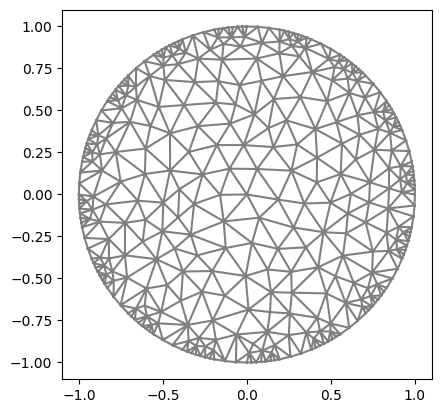
\includegraphics[scale=0.75]{figuras/malha.png}
    \label{fig:malha}
\end{figure}

No método de discretização utilizado, baseado no chamado Método de Elementos Finitos, as funções serão aproximadas por certos espaços de funções com dimensão finita, gerados por tipos de funções especiais. Desse modo, as funções a princípio definidas em um domínio com infinitos pontos, podem ser representadas como um vetor de coeficientes de uma combinação linear. Em particular, para a TIE são utilizados dois espaços: o gerado por funções características, e o gerado por funções afim por partes.

Para o primeiro tipo, consideramos as funções características $\chi_{T_j}$ de cada triângulo $T_j$, as quais indicam se os pontos estão no triângulo $T_j$ correspondente, tendo valor $1$ caso afirmativo e valor $0$ caso contrário. Estas são definidas em $\Omega$ e dadas por:

\begin{equation}
    \chi_{T_j} (x) = \begin{cases}
        1, x \in T_j , \\
        0, x \notin T_j.
    \end{cases}
\end{equation}

No problema específico da TIE, trataremos as condutividades $\gamma$ como funções do espaço gerado por funções características dos triângulos que compõem a triangulação. Isto é, dadas as funções características $\chi_{T_1}, \dots, \chi_{T_N}$ de cada triângulo da malha construída, consideramos que a condutividade é uma função $\gamma \in V_1 = span\{\chi_{T_1}, \dots,\chi_{T_N}\}$ no espaço gerado pelas funções características, podendo assim ser representada na forma:

\begin{equation} \label{eq:gamma-expansao}
    \gamma = \gamma_1 \chi_{T_1} + \dots + \gamma_N \chi_{T_N},
\end{equation}
onde $\gamma_1, \dots, \gamma_N \in \R$ são coeficientes específicos para cada função $\gamma$.

O segundo espaço consiste em funções contínuas afins em cada triângulo. Uma base para esse espaço é composto das funções $v_i$ tais que para cada vértice $P_i$
\begin{equation}
    v_i (P_j) = \begin{cases}
        1, i=j , \\
        0, i \neq j
    \end{cases}
\end{equation}
e são afins dentro de cada triângulo. Essencialmente, é definida uma função para cada vértice, atingindo valor 1 no vértice correspondente e assumindo valores intermediários linearmente em torno dele. No contexto da TIE, esse espaço de funções será utilizado para aproximação das funções de distribuição do potencial. De mesma forma, consideramos a função $u \in V_2 = span\{v_1, \dots, v_n\}$ no espaço gerado $V_2$ por essas funções indicadoras, de forma que:
\begin{equation}\label{eq:u-expansao}
    u = u_1 v_1 + \cdots + u_K v_K
\end{equation}
sendo $u_1,\dots, u_K\in \R$ coeficientes próprios de cada função $u$.

Com as aproximações de $u$ e $\gamma$ através desses espaços finitos, podemos representá-las por um vetor formado pelas coordenadas respectivas. Isto é, dada $\gamma$ com coordenadas $\gamma_1, \dots, \gamma_N$ como na Equação \eqref{eq:gamma-expansao}, podemos tratar $\gamma$ como um vetor $\overline \gamma \in \R^N$ dado por
\begin{equation}
    \overline \gamma = \left( \gamma_1, \dots, \gamma_N \right).
\end{equation}
Similarmente, trataremos $u$ como um vetor $u \in \R^K$ formado por suas coordenadas no espaço de funções $v_i$, como na Equação \eqref{eq:u-expansao}.


\subsection{Cálculo do Operador Direto}


A seguir, descrevemos como pode ser realizado o cálculo do Operador Direto descrito na Seção \ref{sec:modelo-completo-eletrodos} a partir das técnicas de discretização utilizadas. Conforme descrito na seção citada, dados um domínio $\Omega$ contendo $L$ eletrodos, o operador $F$ associa cada condutividade $\gamma$ a um operador $\Lambda_\gamma$, o qual leva cada padrão de correntes $I \in \R^L$ a um padrão de potenciais medidos $U\in \R^L$ correspondentes. Vimos que este é definido a partir da Equação \eqref{eq:cem-variacional}, dada por:
\begin{equation*}
    \iint_\Omega \gamma (x) \nabla u(x) \cdot \nabla v(x)\diff x + \sum_{l=1}^L \frac{1}{z_l}\int_{e_l} (u-U_l)(v - V_l)\diff s = \sum_{l=1}^L I_l V_l,
\end{equation*}
onde para cada $\gamma$ e cada padrão de correntes $I$ existe um único par $(u,U)$ que soluciona a equação dado qualquer par $(v,V)$ sob as condições definidas. 

Conforme detalhado por \citeonline{santana}, dada $\gamma$ no espaço $V_1$ e $u$ no espaço $V_2$ tendo respectivamente vetores de coordenadas $\overline \gamma\in \R^N$ e $\overline u \in \R^K$, como apresentado na subseção anterior, obter a solução $(u,U)$ para a Equação \eqref{eq:cem-variacional} equivale a solucionar um sistema linear
\begin{equation}\label{eq:variacional-linear}
    A \hat u = \overline{I},
\end{equation}
onde $\hat u \in \R^{K+L}$ é um vetor formado pelo ``empilhamento" do vetor de coordenadas $\overline u$ e do padrão de potenciais $U$, na forma:
\begin{equation}
    \hat u = \begin{pmatrix}
        \overline u \\
        U
    \end{pmatrix} = \begin{pmatrix}
        u_1 \\
        \vdots \\
        u_K \\
        U_1 \\
        \vdots \\
        U_L
    \end{pmatrix}.
\end{equation}
A matriz $A$ e o vetor $\overline I$ são formados a partir de cada lado da Equação~\eqref{eq:cem-variacional}, usando as impedâncias de contato, comprimento dos eletrodos, o vetor de correntes $I$ e o vetor $\overline \gamma$ \cite{santana}. Desse modo, a partir da versão discretizada de $\gamma$, podemos obter o padrão de correntes $U = F(\gamma)I = \Lambda_\gamma I$ a partir da solução $\hat u$ do sistema linear \eqref{eq:variacional-linear}.

Com isso, fixando um certo conjunto de padrões de correntes $\mathfrak I = (I^{(1)}\dots, I^{(l)})$, o operador $F_{\mathfrak I}$ conforme definido na Seção~\ref{sec:modelo-completo-eletrodos} pode ser calculado simplesmente a partir da relação:

\begin{equation}
    F_{\mathfrak I}(\gamma) = \begin{pmatrix}
        F(\gamma) I^{(1)} \\
        \vdots \\
        F(\gamma) I^{(l)}
    \end{pmatrix} = \begin{pmatrix}
        U^{(1)} \\
        \vdots \\
        U^{(l)}
    \end{pmatrix},
\end{equation}
onde o cálculo de cada $F(\gamma)I^{(j)}$ para todo $j \in \{1, \dots, l\}$ é realizado através do método descrito acima.


\subsection{Cálculo da Derivada do Operador Direto}


Como descrito na Seção \ref{sec:modelo-completo-eletrodos}, o operador $F$ do Modelo Completo de Eletrodos é diferenciável, o que faz também o Operador Direto $F_{\mathfrak I}$ diferenciável. Isso se torna de grande interesse para alguns dos métodos discutidos no Capítulo \ref{cap}, em especial os de Newton-Inexato. Com isso, podemos tentar obter métodos de trabalhar computacionalmente com a derivada do operador, ou ao menos as derivadas direcionais dado um vetor qualquer. Descrevemos a seguir como é realizado o cálculo da derivada desse operador, a partir das funções discretizadas.

Inicialmente, fixamos um conjunto de $l$ padrões correntes $I^{(1)},\dots, I{(l)}\in \R^L$ linearmente independentes. A partir disso, definimos para cada corrente $I^{(j)}$, com $j \in\{1, \dots, l\}$, o operador $F_j$ dado por
\begin{equation*}
    F_j(\gamma) = F(\gamma) I^{(j)}.
\end{equation*}
Desse modo, a partir do vetor de padrões de correntes $\mathfrak I = (I^{(1)}, \dots, I^{(l)}) \in \R^{l \times L}$, temos que:
\begin{equation}
    F_{\mathfrak I} (\gamma)  = \begin{pmatrix}
        F(\gamma) I^{(1)} \\
        \vdots \\
        F(\gamma) I^{(l)}
    \end{pmatrix} = 
    \begin{pmatrix}
        F_1(\gamma) \\
        \vdots \\
        F_l(\gamma)
    \end{pmatrix}.
\end{equation}

Note que, sendo $F$ diferenciável, segue que $F_j$ é diferenciável para todo $j \in \{1, \dots, l\}$, consequentemente tornando o Operador Direto $F_{\mathfrak I}$ também diferenciável. 

\citeonline{santana} detalha que dada uma função $\eta: \Omega \to \R$ em um espaço apropriado, calcular $F_j'(\gamma)\eta$, a derivada de $F_j$ em $\gamma$ aplicada em uma na direção $\eta$, equivale a obter a solução de uma equação variacional similar à Equação~\eqref{eq:cem-variacional}. Com as funções devidamente discretizadas, análogo ao desenvolvido para cálculo do Operador Direto, essa equação variacional é transformada em um sistema linear na forma

\begin{equation}
    A \hat \omega  = b,
\end{equation}
onde a matriz $A$ é a mesma do sistema \eqref{eq:variacional-linear} e o vetor $b$ é obtido a partir da versão discretizada de $\eta$. A solução $\hat \omega \in \R^{K +L}$ é dada na forma
\begin{equation} \label{eq:solucao-derivada-variacional}
    \hat \omega  = \begin{pmatrix}
        \omega_1 \\
        \vdots \\
        \omega_K \\
        \mathcal W_1 \\
        \vdots \\
        \mathcal W_L
    \end{pmatrix},
\end{equation}
onde o bloco $\mathcal{W}^{(j)} = (\mathcal W_1, \dots, \mathcal W_L)\in \R^L$ corresponde justamente a $F_j'(\gamma) \eta$. Isto é, 
\begin{equation}
    F_j'(\gamma) \eta = \mathcal{W}^{(j)}.
\end{equation}

Com isso, podemos calcular ainda $F_{\mathfrak I}'(\gamma) \eta$ visto que:
\begin{equation}
   F_{\mathfrak I}'(\gamma) \eta = \begin{pmatrix}
        F_1'(\gamma)\eta \\
        \vdots \\
        F_l'(\gamma)\eta
    \end{pmatrix} = \begin{pmatrix}
        \mathcal W^{(1)} \\
        \vdots \\
        \mathcal W^{(1)}
    \end{pmatrix}.
\end{equation}

Portanto, dada uma função $\eta$ com a mesma discretização utilizada para $\gamma$ descrita no início da seção, podemos calcular a derivada de $F_{\mathfrak I}$ em uma certa direção $\eta$ resolvendo sistemas lineares, obtidos a partir de determinadas equações variacionais.

Utilizando esse método, \citeonline{santana} mostra que ainda é possível calcular a Jacobiana de $F_{\mathfrak I}(\gamma)$ para uma $\gamma$ qualquer, a qual é dada por

\begin{equation}
    F_{\mathfrak I}'(\gamma) = \begin{pmatrix}
        F_1'(\gamma) \chi_{T_1} & \cdots & F_1'(\gamma) \chi_{T_1} \\
        \vdots & \ddots & \vdots \\
        F_l'(\gamma) \chi_{T_1} & \cdots & F_l'(\gamma) \chi_{T_N}
    \end{pmatrix},
\end{equation}
sendo $\chi_{T_j}$ a função característica em cada triângulo $T_j$, mostrando ainda um método otimizado para cálculo de cada componente nessa matriz, necessitando de menos soluções de sistemas lineares.

\vspace{1em}

Nesta seção, descrevemos de que forma o Modelo Completo de Eletrodos da TIE pode ser tratado computacionalmente e implementado por meio de métodos numéricos. Conforme comentado anteriormente, este trabalho não possui o intuito de explorar os aspectos teóricos da implementação computacional, sendo, portanto, tratada mais brevemente. Desse modo, recomenda-se para mais detalhes em torno da implementação computacional a consulta nos trabalhos já citados, em especial o de \citeonline{santana}. Por fim, para os experimentos executados no restante deste Capítulo, será utilizada uma biblioteca desenvolvida em Python por \citeonline{hafemann} que provém ferramentas para realizar as operações e cálculos descritos acima, cujos detalhes em torno da implementação podem ser vistos em sua documentação \footnote{Disponível em: \url{https://hafemanne.github.io/FEIT\_CBM34/}}.


\section{Experimentos com Dados Sintéticos}

Na seguinte seção, realizamos diferentes experimentos utilizando dados sintéticos, gerados por funções artificiais pré-definidas. Em situações práticas, não se conhece precisamente a função da condutividade elétrica $\gamma: \Omega \to \R$ que se quer reconstruir. Logo, pode-se ter apenas uma estimativa do erro cometido por uma aproximação $\gamma_n$ gerada pelos métodos de regularização, não se tendo o erro exato. 

Entretanto, nosso intuito nessa seção é justamente definir algumas funções de condutividade, gerar os dados de potenciais através delas para, a seguir, resolver o Problema Inverso e ter uma medição mais precisa do erro obtido em cada método. Com isso, conseguimos, ao menos na situação controlada, medir o quão precisas são as aproximações obtidas pelos métodos.

Começamos inicialmente gerando os dados de potenciais, a partir de algumas funções que serão definidas como solução conhecida que se deseja reconstruir. Em seguida, comparamos as soluções obtidas por diferentes métodos através de alguns cenários diferentes. Primeiramente, vemos como cada método se comporta para diferentes níveis de ruído em uma mesma função. Em seguida, analisamos as reconstruções obtidas para cada solução pré-definida. 

Os métodos selecionados para comparação serão os métodos de Landweber (LW), Levenberg - Marquadt (LM), REGINN com iteração interna Gradiente (NG), e REGINN com iteração interna de Tikhonov (NT).


\chapter{Conclusão}
\section{Trabalhos futuros}

% % % % % % % % % % % % % % % % % % % % % % % % % % % % % %
% % % % % % % % % E ELE TERMINA AQUI % % % % % % % % % %  %
% % % % % % % % % % % % % % % % % % % % % % % % % % % % % %

% % % % % % % % % % % % % % % % % % % % % % % % % % % % % %
% % % % % % % % % % % REFERÊNCIAS % % % % % % % % % % % % %
% % % % % % % % % % % % % % % % % % % % % % % % % % % % % %
\bibliographystyle{abntex2-alf}
\bibliography{refs.bib}
% % % % % % % % % % % % % % % % % % % % % % % % % % % % % %
% % % % % % % % % FIM - REFERÊNCIAS % % % % % % % % % % % %
% % % % % % % % % % % % % % % % % % % % % % % % % % % % % %
\end{document}